% !Mode:: "TeX:UTF-8"
%% Thesis Template of Yanshan University
%% for using YSUthesis package with XeLaTeX
% 2021年3月16日
%% 文档参数配置开始:
%%===========================%
\expandafter\def\csname CTEX@spaceChar\endcsname{\hspace{1em}}
\documentclass[openany]{YSUthesis}
%  showtypeinfo 显示扉页的LaTeX版本信息,去掉即可隐藏版本信息。
%  openany      可以去掉章节起始页必须为奇数页的限制,使章节连续,不出现空白页。
%  推荐的编译顺序为:XeLaTeX > BibTeX > XeLaTeX > XeLaTeX,
%  这样可以生成正确的参考文献和交叉引用链接。

%  设置图形文件的搜索路径。支持图形格式:pdf; png; jpg.
\graphicspath{{chapter/}{figures/}}

%  执行下面的命令可以取消PDF文件中的链接颜色,使用 Adobe Acrobat Reader 查看
%  时,链接可能会有边框,但是在打印时不会出现。
%\hypersetup{colorlinks=false}

% 启用以下这段代码可以让你更改目录的缩进,以备学院有特殊要求。
%\usepackage{titletoc}
%\titlecontents{chapter}[4\ccwd]{}
%                {\bf\contentslabel{4\ccwd}}
%                {\hspace{-4\ccwd}\bf}
%                {\titlerule*[5pt]{.}\contentspage}
%\titlecontents{subsection}[68pt]{}
%                {\contentslabel{40pt}}
%                {\hspace{-4\ccwd}}
%                {\titlerule*[5pt]{.}\contentspage}
\makeatletter   %mzhy55
\renewcommand*\l@chapter{\@dottedtocline{1}{0em}{3.5em}}%使英文章标题缩进,原来是0em
\renewcommand*\l@section{\@dottedtocline{1}{15pt}{2.0em}}
\renewcommand*\l@subsection{\@dottedtocline{2}{24pt}{2.5em}}%使英文目录的小节标题左移,对齐,原来是{2}{24pt}{24pt}
\renewcommand*\l@subsubsection{\@dottedtocline{3}{42pt}{36pt}}
%\renewcommand*\l@paragraph{\@dottedtocline{4}{48pt}{48pt}}
%\renewcommand*\l@subparagraph{\@dottedtocline{5}{60pt}{60pt}}
\makeatother    %mzhy55

% 选择数学字体,xits-math.otf为类Times字体,Cambria Math与Office2010数学公式格式相同。
\setmathfont{XITSMath}
%%===========================%
%% 文档参数配置结束

\usepackage{makecell}
\usepackage{titlesec}
\usepackage{titletoc}%%%%%mzhy55 解决目录中章标题的黑体问题
\titlecontents{chapter}[0pt]{\bf\vspace{0mm}}
{\thecontentslabel\hskip.5em}{}
{\titlerule*[0.45pc]{.}\contentspage}
%%%%%%%%%%%%%%%%%%%%%%%%%%%mzhy55 解决目录中章标题的黑体问题
%\addbibresource{tex.bib}
%% 文档正式开始
%============================%
\begin{document}

%%调整公式与正文间距离,调整空白大小命令:
\setlength{\abovedisplayskip}{4pt} %%% 4pt 个人觉得稍妥,可自行设置
\setlength{\belowdisplayskip}{4pt}

% 以下为封面部分
%----------------------------%
  % 中文封面内容

  \classification{O469}                            % 中图分类号,注意,此项要自己查,更改!!!
  \UDC{530}                                          % UDC,注意,此项要自己查,更改!!!
  \title{两轮平衡小车控制系统设计与实现}                           % 论文题目
  \author{石殿鹏}                                   % 作者姓名,注意:姓在前,名在后!!!
  \advisor{胡硕\, 讲师}                         % 导师姓名,注意:姓在前,名在后,若是“副教授”,加上“副”字!!!
  \degree{本科生}                                % 申请学位
  \major{过程控制}                               % 专业,注意,此项要以自己实际情况修改!!!
  \institute{电气工程学院}                                 % 所在单位
  \defenddate{2021年6月}                        % 答辩日期,注意:要依实际答辩时间修改!!!
  \school{燕山大学}                                 % 院校名称

  % 英文封面内容
  \enstatement{Condensed Physics}                     % 学科或领域%{Science}
  \entitle{RESEARCH OF ...... BASED ON ......}      % 英文题目,所有字母大写
  \enauthor{Zhang Moumou}                              % 作者英文姓名,注意:姓在前,名在后!!!
  \enadvisor{Professor Wang Moumou}                % 导师英文姓名,注意:姓在前,名在后,若是“副教授”,加上“Associate”词!!!
  \enschool{Yanshan University}                         % 院校英文名称
  \enathdate{May, 2020}                                    % 英文答辩日期,注意:要依实际答辩时间修改!!!

\makeatletter    %%%%%%%mzhy55
\newcommand\makecover{%
  \cleardoublepage
  \thispagestyle{empty}
  \begin{center}
    
\includegraphics[width=9.0cm]{ysulogo}\\
    \vspace*{1.5cm}
    {\zihao{-0}
    %\ziju{0.5}
    \heiti{本科生毕业设计(论文)}}\\
    \vspace*{0.5cm}
    %{\zihao{-2} DOCTORAL DISSERTATION}\\
    \vspace*{3cm}
    \begin{tabular}{p{3cm}p{9cm}}
      \zihao{-2}{\heiti 论文题目} & \zihao{-2}{\kaishu\CAST@value@title}
    \end{tabular}
    \vfill
    \renewcommand{\arraystretch}{2}
    \begin{tabular}{p{3cm}p{9cm}}
      \zihao{-2}{\heiti 作者姓名} & \zihao{-2}{\kaishu\CAST@value@author} \\
      \zihao{-2}\heiti\begin{CJKfilltwosides}{2.6cm}专业\end{CJKfilltwosides} & \zihao{-2}{\kaishu\CAST@value@major}  \\
      %\multicolumn{1}{@{}c@{}}
     % {\begin{tabular}{p{1.5cm}p{1.5cm}}
     %   \zihao{-2}{\heiti 专} & \zihao{-2}{\heiti 业}
      %\end{tabular}}& \zihao{-2}{\kaishu\CAST@value@major}  \\
      %\zihao{-2}{\heiti 专 \qquad 业} & \zihao{-2}{\kaishu\CAST@value@major}  \\
      \zihao{-2}{\heiti 指导教师} & \zihao{-2}{\kaishu\CAST@value@advisor}
    \end{tabular}\\
    \vspace*{2cm}
    \zihao{-2}\songti\textbf{2021年6月}%%%第一页上的日期,根据实际答辩时间填写,  mzhy55
  \end{center}
\clearpage
\if@twoside
\thispagestyle{empty}
\cleardoublepage
\fi}
\makeatother    %%%%%%%mzhy55

  % 生成封面
  \makecover

  % 生成中文封里
  \maketitle

  % 生成英文封里
  %\makeenglishtitle

  % 生成原创性声明
  %\makelicense


% 以下为前言部分
%----------------------------%
\frontmatter
\pagenumbering{Roman}

  % 摘要
  % !Mode:: "TeX:UTF-8"
%%%%%%% 以下内容不要修改!!! mzhy55
\makeatletter
\fancypagestyle{plain}{%
  \fancyhf{}%
  \renewcommand{\headrulewidth}{0pt}%
  \renewcommand{\footrulewidth}{0pt}%
%  \renewcommand{\headrule}{}
  \fancyhead[CE]{{\zihao{5} 燕山大学\CAST@value@degree 毕业设计(论文)}}
  \fancyhead[CO]{\zihao{5} 摘\ \ 要}
  \fancyfoot[C]{{\zihao{-5} -~\thepage~-}}
  }
  \pagestyle{fancy}%%%%% 页眉 mzhy55
  \fancyhf{}
  \fancyhead[CE]{{\zihao{5} 燕山大学\CAST@value@degree 毕业设计(论文)}}
  \fancyhead[CO]{{\zihao{5} 摘\ \ 要}}
  \fancyfoot[C]{{\zihao{-5} -~\thepage~-}}
\makeatother
%%%%%%% 以上内容不要修改!!! mzhy55

\begin{abstract}
摘要是论文内容的高度概括,应具有独立性和自含性,即不阅读论文的全文,就能通过摘要了解整个论文的必要信息。摘要应包括本论文研究的目的、理论与实际意义、主要研究内容、研究方法等,重点突出研究成果和结论。

摘要的内容要完整、客观、准确,应做到不遗漏、不拔高、不添加。摘要应按层次逐段简要写出,避免将摘要写成目录式的内容介绍。摘要在叙述研究内容、研究方法和主要结论时,除作者的价值和经验判断可以使用第一人称外,一般使用第三人称,采用“分析了……原因”、“认为……”、“对……进行了探讨”等记述方法进行描述。避免主观性的评价意见,避免对背景、目的、意义、概念和一般性(常识性)理论叙述过多。

摘要需采用规范的名词术语(包括地名、机构名和人名)。对个别新术语或无中文译文的术语,可用外文或在中文译文后加括号注明外文。摘要中不宜使用公式、化学结构式、图表、非常用的缩写词和非公知公用的符号与术语,不标注引用文献编号。

摘要的字数(以汉字计),硕士学位论文一般为500-650字,博士学位论文为900-1200字,均以能将规定内容阐述清楚为原则,文字要精练,段落衔接要流畅。摘要页不需写出论文题目。

英文摘要与中文摘要的内容应完全一致,在语法、用词上应准确无误,语言简练通顺。中文摘要在前,英文摘要在后。


\end{abstract}

\begin{keywords}
关键词1;关键词2;关键词4;关键词4 \qquad(关键词是供检索用的主题词条。关键词应集中体现论文特色,反映研究成果的内涵,具有语义性,在论文中有明确的出处,并应尽量采用《汉语主题词表》或各专业主题词表提供的规范词,应列取3-8个关键词,按词条的外延层次从大到小排列。)
\end{keywords}

%%%%%%%%%%%%%%%%%%%%%%%%%%%%%%%%%%%%%%%%%%%%%%%%%%%%%%%%%%%%%%%%%%%%%%%%%%%%%%%%%%%%%%%%%%%%
\clearpage
\phantomsection
%mzhy55注释掉,中文摘要后边没有空白页,英文摘要接着,不管在奇数页还是偶数页
%%%%%%%%%%%%%%%%%%%%%%%%%%%%%%%%%%%%%%%%%%%%%%%%%%%%%%%%%%%%%%%%%%%%%%%%%%%%%%%%%%%%%%%%%%%%

%%%%%%% 以下内容不要修改!!! mzhy55
\newpage\ \vspace{-2.5em}
\begin{center}
\zihao{-2}\textbf{Abstract}
\end{center}
\addcontentsline{toc}{chapter}{\bf ABSTRACT}%%%%%目录 mzhy55

\makeatletter
  \fancypagestyle{plain}{%
  \fancyhf{}%
  \renewcommand{\headrulewidth}{0pt}%
  \renewcommand{\footrulewidth}{0pt}%
%  \renewcommand{\headrule}{}
  \fancyhead[CE]{{\zihao{5} 燕山大学\CAST@value@degree 毕业设计(论文)}}
  \fancyhead[CO]{\zihao{5} Abstract}
  \fancyfoot[C]{{\zihao{-5} -~\thepage~-}}
  }
  \pagestyle{fancy}%%%%% 页眉 mzhy55
  \fancyhf{}
  \fancyhead[CE]{{\zihao{5} 燕山大学\CAST@value@degree 毕业设计(论文)}}
  \fancyhead[CO]{{\zihao{5} Abstract}}
  \fancyfoot[C]{{\zihao{-5} -~\thepage~-}}
\makeatother
%%%%%%% 以上内容不要修改!!! mzhy55


This is the abstract of your paper and it should be ...

This is the abstract of your paper and it should be This is the abstract of your paper and it should be ...This is the abstract of your paper and it should be ...


\begin{englishkeywords}
Photonic crystal fiber; dispersion; birefringence; genetic algorithm; finite element method; terahertz
\end{englishkeywords}

\cleardoublepage%这一行保证了目录页从奇数页开始!

%%%%%%% 以下内容不要修改!!! mzhy55
\makeatletter
\fancypagestyle{plain}{%
  \fancyhf{}%
  \renewcommand{\headrulewidth}{0pt}%
  \renewcommand{\footrulewidth}{0pt}%
%  \renewcommand{\headrule}{}
  \fancyhead[CE]{{\zihao{5} 燕山大学\CAST@value@degree 毕业设计(论文)}}
  \fancyhead[CO]{\zihao{5} \nouppercase \leftmark}
  \fancyfoot[C]{{\zihao{-5} -~\thepage~-}}
  }
\pagestyle{fancy}
  \fancyhf{}
  \fancyhead[CE]{{\zihao{5} 燕山大学\CAST@value@degree 毕业设计(论文)}}
  \fancyhead[CO]{{\zihao{5} \nouppercase \leftmark}}
  \fancyfoot[C]{{\zihao{-5} -~\thepage~-}}
\makeatother
%%%%%%% 以上内容不要修改!!! mzhy55


  % 目录
  \tableofcontents
  % 表格目录
  %\listoftables
  % 插图目录
  %\listoffigures


% 以下为正文部分
%----------------------------%
\mainmatter
  % !Mode:: "TeX:UTF-8"
\chapter{快速入门}\label{chap:introduction}


本模板的意义是为了让从未接触过\LaTeX 的新手能尽快的上手,熟悉
本模板的使用。因此本文介绍的大部分内容都将以实例的形式给出,您
可以通过目录快速检索感兴趣的内容。作为一个学文论文作者,你的主
要精力应该是论文的内容而不是论文的格式。字体字号对齐方式是否有
背题图和图注是否在同一页参考文献作者是否缩写期刊名是否缩写——
这些不应该成为一个即将具有博士学位的人花费大量精力去考虑的问题。
这也是本模板要解决的问题。

本说明的结构安排如下:第 \ref{chap:introduction} 章是一篇简易教程,完整的示例了论文的
一章可能会遇到的各种问题如插图、公式、图形引用、公式引用和文献
的插入及引用。第 \ref{chap:figures}章是关于插图的进阶内容,会涉及到图形的不同排
列形式,图形的大小缩放等。第 \ref{chap:table}章是关于表格的内容,涉及如何插入表格,
科技文献常用的三线表以及跨页长表格等问题。第 \ref{chap:equ} 章是关于公式的进阶内容,涉及公式
的编号、对齐、矩阵和方程组的编写等问题。第 \ref{chap:bib}章是关于参考文献,
涉及文献的压缩引用,排序等。%第 \ref{chap:chap-5}章则介绍了在文章内加入计算机程序源代码的方法。
第 \ref{chap:unit}章介绍输入数字和物理量的方法。

\section{高楼大厦始于一砖一瓦}\label{section1-1}
简单的说,\LaTeX 是一种对文字进行排版处理的程序语言,尽管它的功
能不仅限于此。它与我们常用的Microsoft Word在使用上有较大的区
别。例如我们在MSWord中输入标题时,先输入标题文字,如“绪论”,
然后将其选中,选择MSWord中的“章标题”样式。这是在已经定义好
了章标题样式的前提下。如果从未听说过样式或者没有使用过MSWord样
式的同学,可能会采取更为繁琐的操作,例如分别设定字体,字号,大
纲级别,缩进,对齐方式和自动编号等等。在\LaTeX 中,是这样输入
章标题的:\\[2pt]
\hspace*{5cm}\verb|\chapter{绪论}|\\[2pt]
仅此而已。这里的\verb|\chapter|是一个\textbf{命令},它告诉\LaTeX
“绪论”是章标题,然后\LaTeX 会按照预先定义好的章标题格式来对其
进行处理——这不是我们应该关心的内容。同样,你可以使用
\verb|\section{课题背景}|、\verb|\subsection{理论基础}|和
\verb|\subsubsection{公式推导}|
来告诉\LaTeX 这些分别是节标题、
条标题和款标题。\LaTeX 会自动对它们进行格式的设置,并且会自动
为你生成编号。

而图形的插入通常则是通过以下形式:
\begin{verbatim}
\begin{figure}
 
\includegraphics{ysulogo}
\end{figure}
\end{verbatim}
其中ysulogo为插图的文件名,不包含后缀名(\XeLaTeX 支持PDF, PNG, JPG 格式)。与命令不同,这里使用了\\
\verb|\begin{figure}|
和
\verb|\end{figure}|\\
这一对命令来构成一个\textbf{环境}。使用本模板完成学位论文时将会经常
用到命令与环境。一般使用者只要能区分开二者即可,其实只要完成论文的
第一幅插图,后续的插图可以将原来的插图环境复制并稍加修改即可。

\section{一个完整的章节实例}\label{section1-2}
下边我们使用命令与环境的概念,完成一个迷你章节的例子。

进入YSUthesis文件夹,打开主文件template.tex。进入chapter文件夹,
打开chap-intro.tex文件。该文件对应论文的第一章“绪论”。然后输入如下内容:
\begin{verbatim}
% !Mode:: "TeX:UTF-8"
\chapter{绪论}
我是绪论中的正文文本。

\section{课题背景}
我要使用引用命令为我的文章引用文献:
\ldots加速度为\SI{12345}{\square\micro\meter\per\nano\second},
是一般加速度的\num{1.2345e3}倍\supercite{Yablonovitch1987},
误差\SI{+-2e-6}{\square\micro\meter\per\nano\second}。

\subsection{该小节插图}
这里我要使用图形环境插图。注意该插图拥有中英双语图注和自动生成的图形编号。
同时我要引用该图形:该图的编号是 \ref{fig-pcf}。
\begin{figure}[hptb]
\centering
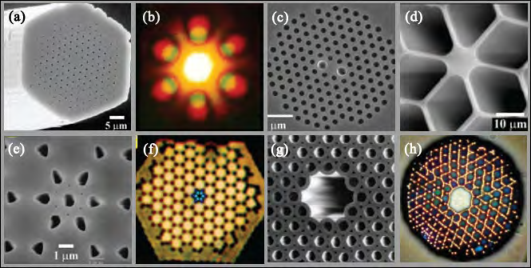
\includegraphics{chp-1_pcf}
\FigureBiCaption{形式多样的光子晶体光纤}{英文图题}\label{fig-pcf}
\end{figure}

\subsection{该小节插入公式}
我还要使用公式环境插入公式。注意公式是自动居中编号。同时我也要引用该公式,
该公式的编号是\eqref{equ-sample}
\begin{equation}\label{equ-sample}
\sum_{i=1}^n\sin\beta_i^2+\int_a^b\frac{D}{c}\,\mathrm{d}x=0.
\end{equation}

\section{本章小结}
以上为本章的所有内容。
\end{verbatim}
保存该文件。切换到template.tex主文件,依次执行菜单``TeX"下的``XeLaTeX" 
- ``BibTeX" - ``XeLaTeX" - ``XeLaTeX",(这些步骤也可以通过工具栏上的
按钮完成)。之后会在主目录下自动生成PDF文件,您不妨亲自动手试试看!
生成的参考文献如图 \ref {fig-ctt}所示。
\begin{figure}[hptb]
 \centering
 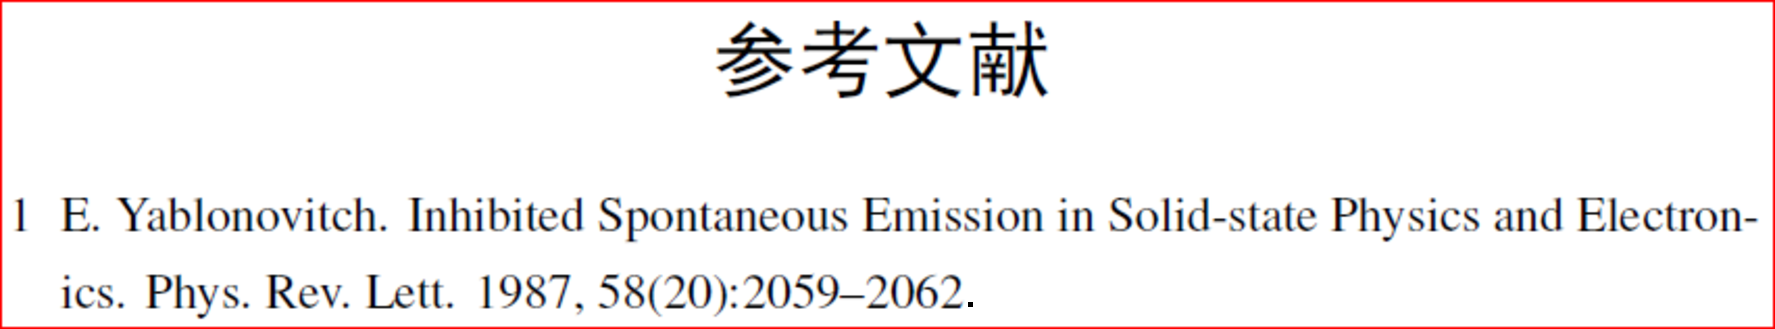
\includegraphics[width=\linewidth]{citation}
\FigureBiCaption{自动生成的参考文献\label{fig-ctt}}
{References are generated automatically}\vspace{0.3em}
\end{figure}

\section{章节条款标题}\label{section1-3}
论文的框架分为:章节条款等,分别由下列一些命令生成。由\verb|\chapter{}|生成章标题
,由 \\ \verb|\section{}|生成节标题,由\verb|\subsection{}| 生成条标题,
   由 \verb|\subsubsection{}| 生成款标题。

\subsection{条标题}\label{section1-3-1}
论文的框架分为:章节条款等,分别由下列一些命令生成。由\verb|\chapter{}|
生成章标题,由 \\ \verb|\section{}|生成节标题,由\verb|\subsection{}| 生
成条标题,由 \verb|\subsubsection{}| 生成款标题。

\subsubsection{款标题}\label{section1-3-1-1}
论文的框架分为:章节条款等,分别由下列一些命令生成。
由\verb|\chapter{}| 生成章标题,由\\ \verb|\section{}|生成节标题,
由\verb|\subsection{}| 生成条标题, 由命令\verb|\subsubsection{}| 生
成款标题。


\section{解决pdf文件复制出现乱码问题}\label{section1-4}
\begin{verbatim}
以下是解决pdf文件复制乱码问题(方便论文查重,
我已经按照第一种办法做了,如果有个别同学还是不成功,请按照后边方法
,照做一下)!!!下面是另外两种办法,共三种办法!!!
(1) 在YSUthesis.cls的Line142,加上``\setCJKmainfont{新宋体}第一种办法!''
%%上面一行是解决pdf文件复制乱码问题!!!下面是另外两种办法,共三种办法!

(2) 在template.tex文件的\begin{document}前边,加上
``\usepackage{ccmap}删掉前边的注释!为了解决论文查重,
PDF文件复制出现乱码问题,请去掉这行前面的注释,编译完成后,
使用Adobe Acrobat 删掉论文前面多余的两页即可!!!不知道是
什么原因,但是这样可以解决问题,有待大家找到更好的解决办法!!!
这种方法在编译过程中会终止,需要回车一下!!!''

(3) 在template.tex文件的\classification{O226}前边,加上
``为了解决论文查重,PDF文件复制出现乱码问题,请去掉这行前面的注释
,编译完成后,使用Adobe Acrobat 删掉论文前面多余的两页即可!!!
不知道是什么原因,但是这样可以解决问题,有待大家找到更好的解决办法!!!''

\end{verbatim}

注意!第一章不要有``本章小结"!!!


%

  % !Mode:: "TeX:UTF-8"
\chapter{插图}
\label{chap:figures}

插图主要涉及到:单个居中图形;两个并排图形;两个以上的并排或者堆叠的图形;图题;图形的引用;

\section{单个居中图形}\label{section2-1}

大多数情况下,需要插入的图形是单个的时候可以使用如下环境:

\begin{verbatim}
\begin{figure}[hptb!]
 \centering\small
 
\includegraphics[width=0.6\textwidth]{ysulogo}
 \FigureBiCaption{单个居中图形}
 {A single center graphics A single center graphics}\label{ysulogo}%\vspace{0.3em}
\end{figure}

或者

\begin{figure}[hptb!]
 \centering\small
 
\includegraphics[width=0.6\textwidth]{ysulogo}
 \caption{单个居中图形\label{ysulogo}}\vspace{0.3em}
 \begin{minipage}[t]{0.9\textwidth}
 \centering
 {Fig.  \ref{ysulogo} A single center graphics}
 \end{minipage}
\end{figure}
\end{verbatim}
其中的参数“[width=$\backslash$textwidth]”指定图形的宽度0.6倍页宽。两种方式都可以达到最后的效果如图 \ref{ysulogo}所示。个人推荐第一种方式。
\begin{figure}[hptb!]
 \centering\small
 
\includegraphics[width=0.6\textwidth]{ysulogo}
 \FigureBiCaption{单个居中图形}
 {A single center graphics A single center graphics }\label{ysulogo} 
\end{figure}


\section{两个并排图形}\label{section2-2}
下列代码在文中插入两个并排的图形。它使用了一个称作minipage
的环境。在同一行插入两个并排的minipage,每个minipage包含一
个图形。图中minipage的参数“[0.5$\backslash$linewidth]”指定minipage
的宽度是当前正文页面的0.5倍(一半)。而插图命令中的参数
“[width=$\backslash$textwidth]”则是指定插图的宽度为当前minipage的宽
度。如果这个插图命令是在minipage环境外边的话,参数中的
“$\backslash$textwidth”的宽度为当前正文页面的宽度。
\begin{verbatim}
\begin{figure}[htbp!]
\centering
\subfigure{\label{subfigure1}}\addtocounter{subfigure}{-2}
\subfigure[The 1st subfigure caption]{\subfigure[第1个子图标题]
{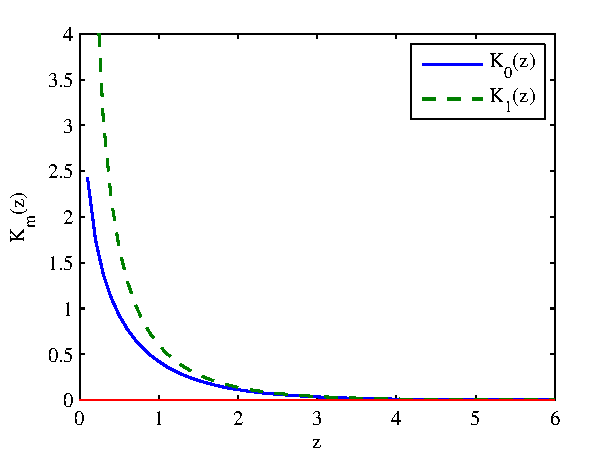
\includegraphics[width=0.46\textwidth]{chp-2_bessel_k}}}%%%%%%%第1个子图
\subfigure{\label{subfigure2}}\addtocounter{subfigure}{-2}
\subfigure[The 2nd subfigure caption]{\subfigure[第2个子图标题]
{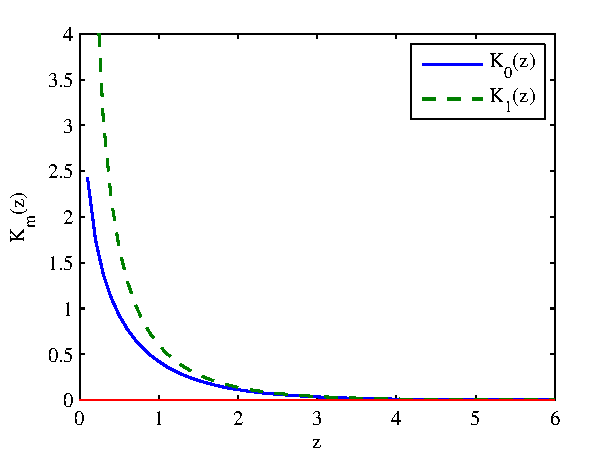
\includegraphics[width=0.46\textwidth]{chp-2_bessel_k}}}%%%%%%%第2个子图
\FigureBiCaption{中文总标题}{The total caption\label{Figure-all}}
\end{figure}

或者

\begin{figure}[hptb!]
  \centering\small
  \begin{minipage}[t]{0.5\linewidth}
    \centering
    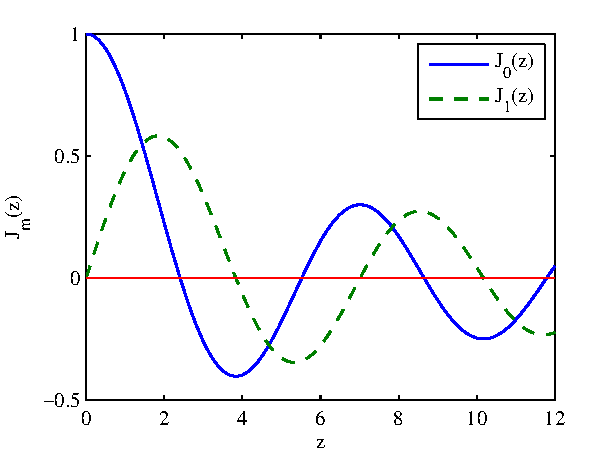
\includegraphics[width=\textwidth]{chp-2_bessel_j}
    (a) 子图a图题\\[0.3em]
    (a) Subfigure a
  \end{minipage}%
  \begin{minipage}[t]{0.5\textwidth}
    \centering
    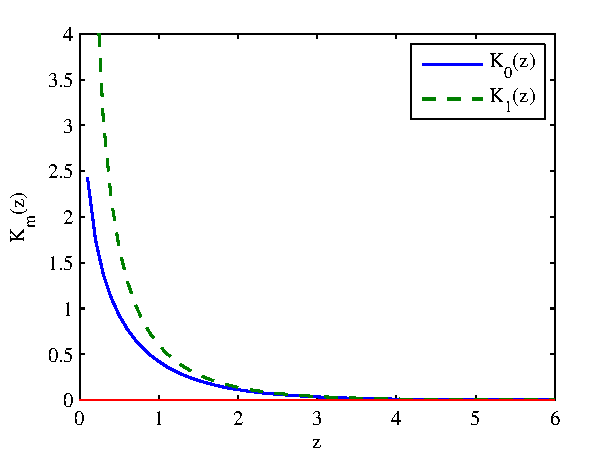
\includegraphics[width=\textwidth]{chp-2_bessel_k}
    (b) 子图b图题\\[0.3em]
    (b) Subfigure b
  \end{minipage}
  \FigureBiCaption{两个并排图形}{Two coordinate graphics}\label{fig-dbfig}
 \end{figure}

或者

\begin{figure}[hptb!]
  \centering\small
  \begin{minipage}[t]{0.5\linewidth}
    \centering
    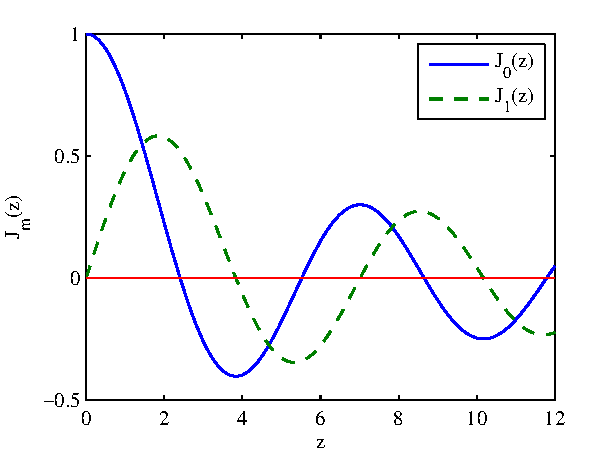
\includegraphics[width=\textwidth]{chp-2_bessel_j}
    (a) 子图a图题\\[0.3em]
    (a) Subfigure a
  \end{minipage}%
  \begin{minipage}[t]{0.5\textwidth}
    \centering
    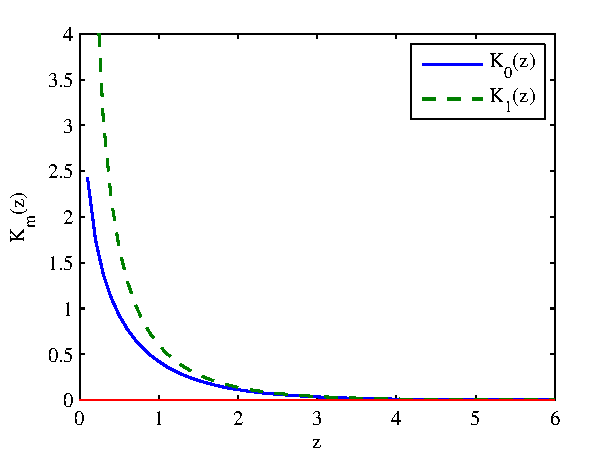
\includegraphics[width=\textwidth]{chp-2_bessel_k}
    (b) 子图b图题\\[0.3em]
    (b) Subfigure b
  \end{minipage}
    \caption{两个并排图形\label{fig-dbfig}}
    \vspace{0.3em}
 \begin{minipage}[t]{0.9\textwidth}
 \centering
 {Fig.  \ref{fig-dbfig} Two coordinate graphics}
 \end{minipage}
 \end{figure}
\end{verbatim}
最终结果如图 \ref{fig-dbfig}所示。
\begin{figure}[htbp!]
\centering
\subfigure{\label{subfigure1}}\addtocounter{subfigure}{-2}
\subfigure[The 1st subfigure caption]{\subfigure[第1个子图标题]
{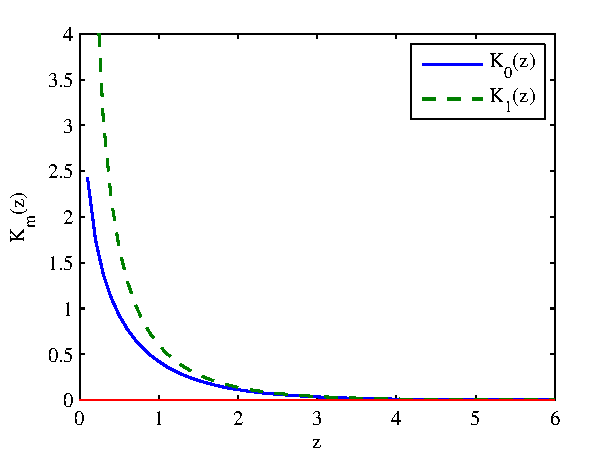
\includegraphics[width=0.46\textwidth]{chp-2_bessel_k}}}%%%%%%%第1个子图
\subfigure{\label{subfigure2}}\addtocounter{subfigure}{-2}
\subfigure[The 2nd subfigure caption]{\subfigure[第2个子图标题]
{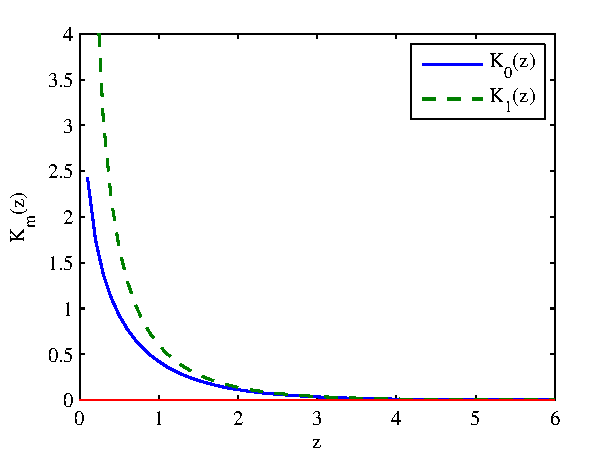
\includegraphics[width=0.46\textwidth]{chp-2_bessel_k}}}%%%%%%%第2个子图
\FigureBiCaption{中文总标题}{The total caption\label{Figure-alll}}
\end{figure}

\begin{figure}[hptb!]
  \centering\small
  \begin{minipage}[t]{0.5\linewidth}
    \centering
    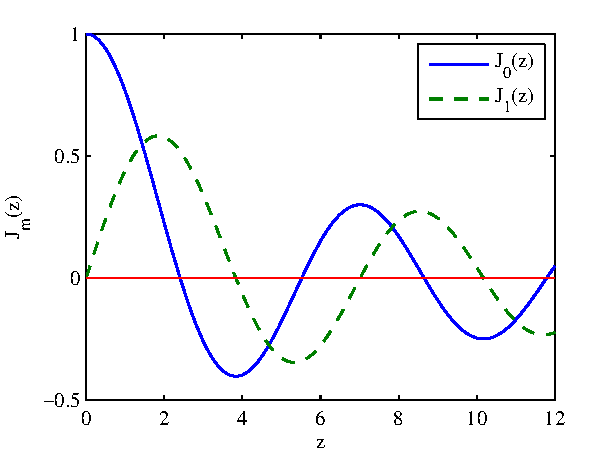
\includegraphics[width=\textwidth]{chp-2_bessel_j}
    (a) 子图a图题\\[0.3em]
    (a) Subfigure a Subfigure a
  \end{minipage}%
  \begin{minipage}[t]{0.5\textwidth}
    \centering
    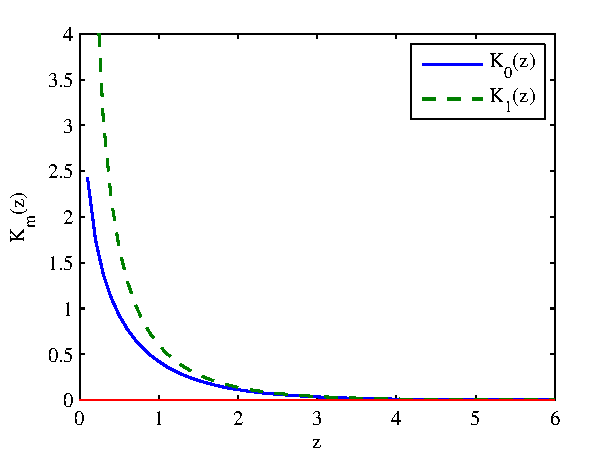
\includegraphics[width=\textwidth]{chp-2_bessel_k}
    (b) 子图b图题\\[0.3em]
    (b) Subfigure b Subfigure b
  \end{minipage}
  \FigureBiCaption{两个并排图形}{Two coordinate graphics}\label{fig-dbfig}
 \end{figure}



\section{两个以上的并排或者堆叠的图形}\label{section2-3}
同样是使用minipage的方法,只不过排列的方式不同。例如4幅堆叠排列的图形。
\begin{verbatim}
\begin{figure}[htbp!]
\centering
\subfigure{\label{subfigure1}}\addtocounter{subfigure}{-2}
\subfigure[The 1st subfigure caption]{\subfigure[第1个子图标题]
{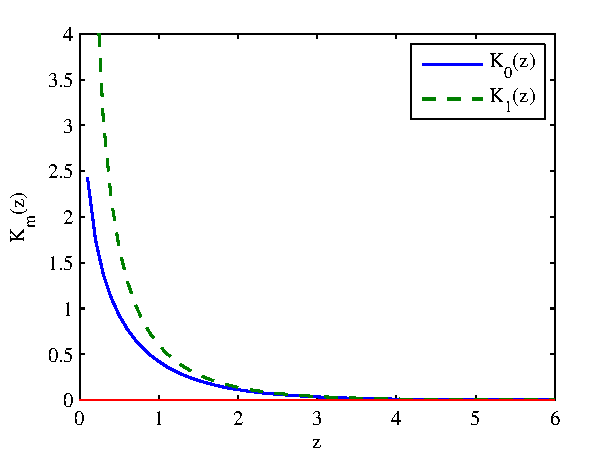
\includegraphics[width=0.46\textwidth]{chp-2_bessel_k}}}%%%%%%%第1个子图
\subfigure{\label{subfigure2}}\addtocounter{subfigure}{-2}
\subfigure[The 2nd subfigure caption]{\subfigure[第2个子图标题]
{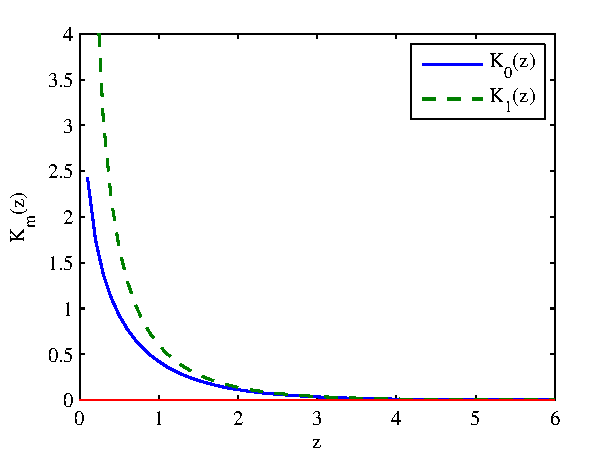
\includegraphics[width=0.46\textwidth]{chp-2_bessel_k}}}\\[-1.5em]%%%%%%%第2个子图
\subfigure{\label{subfigure1}}\addtocounter{subfigure}{-2}
\subfigure[The 3rd subfigure caption]{\subfigure[第3个子图标题]
{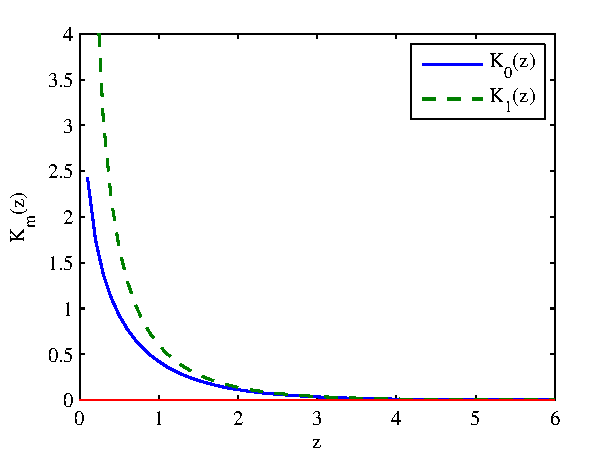
\includegraphics[width=0.46\textwidth]{chp-2_bessel_k}}}%%%%%%%第3个子图
\subfigure{\label{subfigure4}}\addtocounter{subfigure}{-2}
\subfigure[The 4th subfigure caption]{\subfigure[第4个子图标题]
{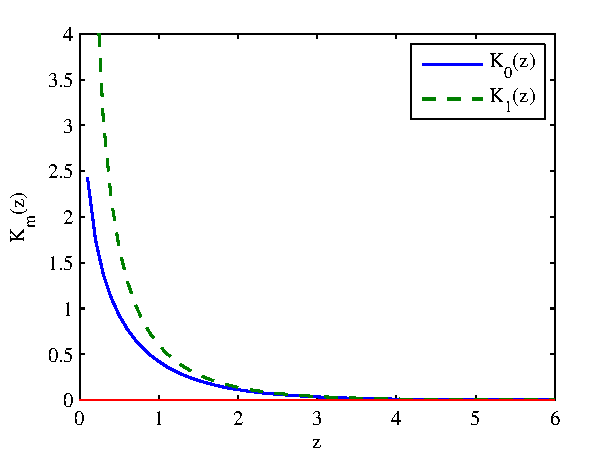
\includegraphics[width=0.46\textwidth]{chp-2_bessel_k}}}%%%%%%%第4个子图\\
\FigureBiCaption{中文总标题}{The total caption\label{Figure-all}}
\end{figure}

或者

\begin{figure}[hptb!]
  \centering\small
  \begin{minipage}[t]{0.5\linewidth}
    \centering
    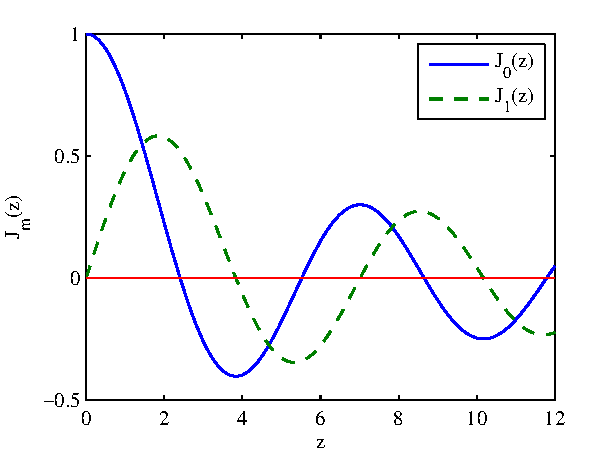
\includegraphics[width=\textwidth]{chp-2_bessel_j}
    (a) 子图a图题\\[0.3em]
    (a) Subfigure a
  \end{minipage}%
  \begin{minipage}[t]{0.5\textwidth}
    \centering
    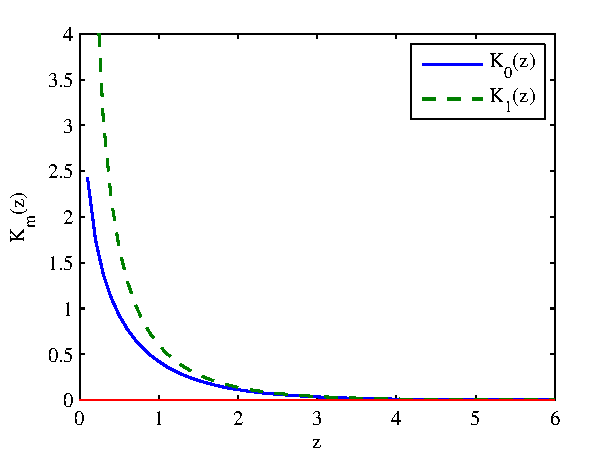
\includegraphics[width=\textwidth]{chp-2_bessel_k}
    (b) 子图b图题\\[0.3em]
    (b) Subfigure b
  \end{minipage}  \\
  \begin{minipage}[t]{0.5\textwidth}
    \centering
    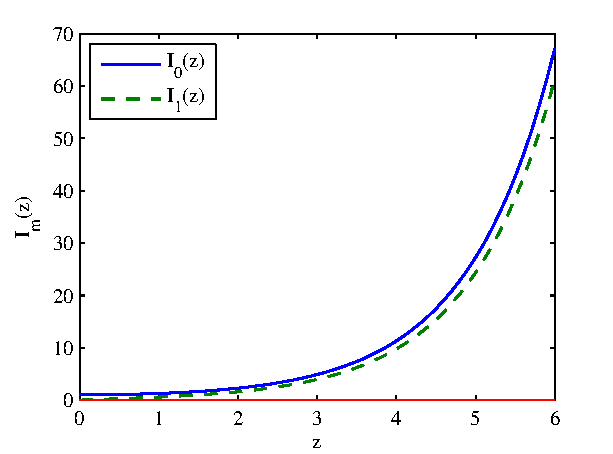
\includegraphics[width=\textwidth]{chp-2_bessel_i}
    (c) 子图c图题\\[0.3em]
    (c) Subfigure c
  \end{minipage}%
  \begin{minipage}[t]{0.5\textwidth}
    \centering
    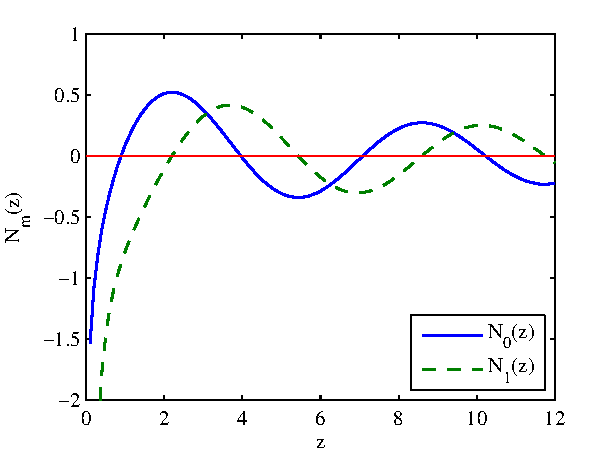
\includegraphics[width=\textwidth]{chp-2_bessel_n}
    (d) 子图d图题\\[0.3em]
    (d) Subfigure d
  \end{minipage}
  \FigureBiCaption{贝塞尔函数}{Bessel function}\label{fig-bessel-function}
\end{figure}
\end{verbatim}
注意其中与一对并排图形不同的地方,加入了换行命令“$\backslash\backslash$”。
最终效果如图 \ref{fig-bessel-function}所示。
\begin{figure}[htbp!]
\centering\small
\subfigure{\label{subfigure11}}\addtocounter{subfigure}{-2}
\subfigure[The 1st subfigure caption]{\subfigure[第1个子图标题]
{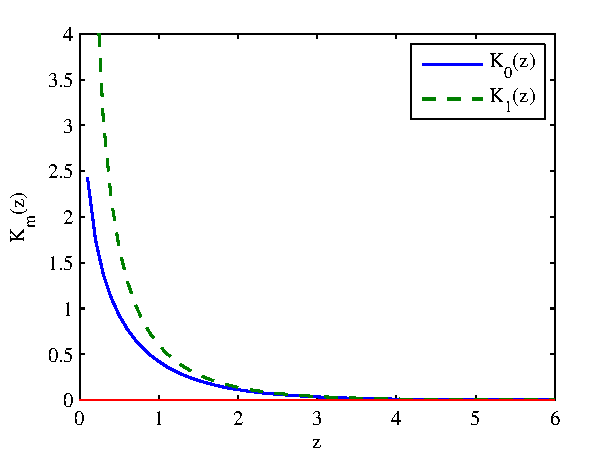
\includegraphics[width=0.46\textwidth]{chp-2_bessel_k}}}%%%%%%%第1个子图
\subfigure{\label{subfigure22}}\addtocounter{subfigure}{-2}
\subfigure[The 2nd subfigure caption]{\subfigure[第2个子图标题]
{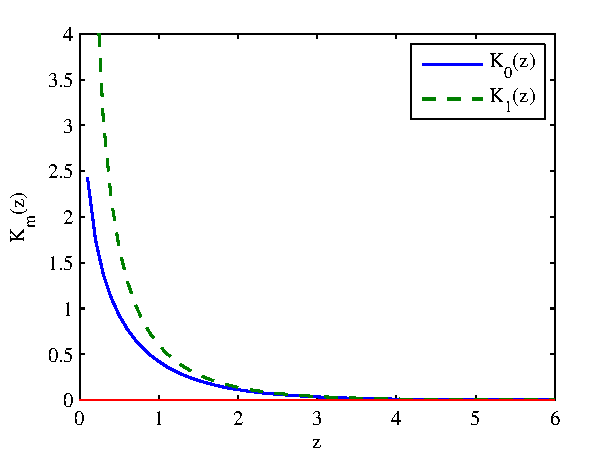
\includegraphics[width=0.46\textwidth]{chp-2_bessel_k}}}\\[-1.5em]%%%%%%%第2个子图
\subfigure{\label{subfigure3}}\addtocounter{subfigure}{-2}
\subfigure[The 3rd subfigure captionThe 3rd subfigure caption]{\subfigure[第3个子图标题第3个子图标题]
{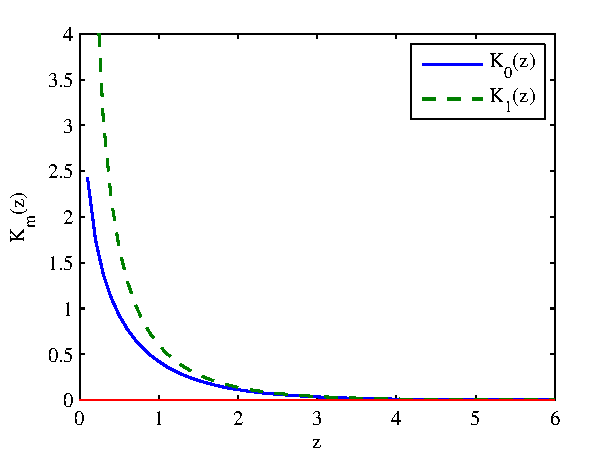
\includegraphics[width=0.46\textwidth]{chp-2_bessel_k}}}%%%%%%%第3个子图
\subfigure{\label{subfigure4}}\addtocounter{subfigure}{-2}
\subfigure[The 4th subfigure captionThe 4th subfigure caption]{\subfigure[第4个子图标题第4个子图标题]
{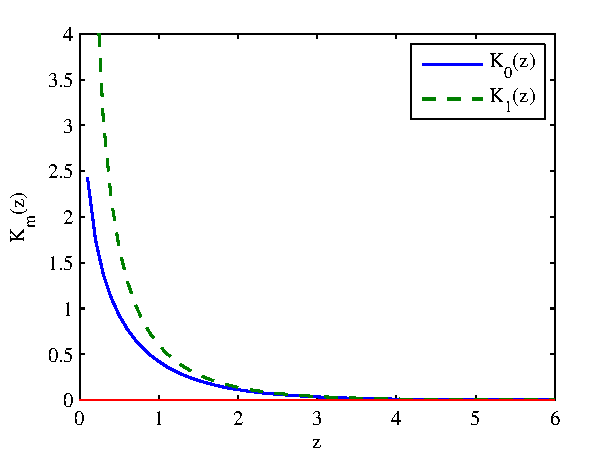
\includegraphics[width=0.46\textwidth]{chp-2_bessel_k}}}%%%%%%%第4个子图\\
\FigureBiCaption{中文总标题}{The total caption\label{Figure-all}}
\end{figure}
\begin{figure}[hptb!]
  \centering\small
  \begin{minipage}[t]{0.5\linewidth}
    \centering
    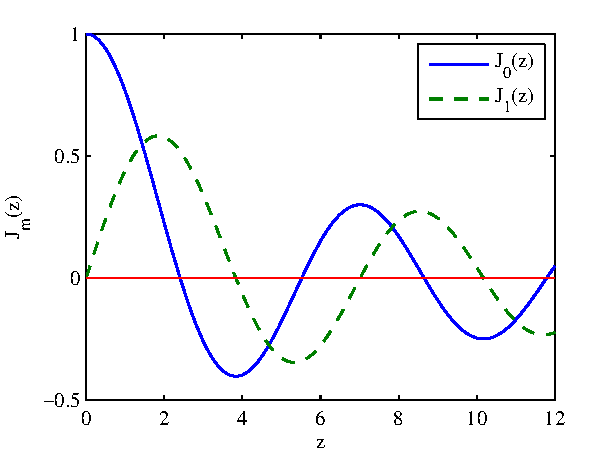
\includegraphics[width=\textwidth]{chp-2_bessel_j}
    (a) 子图a图题\\[0.3em]
    (a) Subfigure a
  \end{minipage}%
  \begin{minipage}[t]{0.5\textwidth}
    \centering
    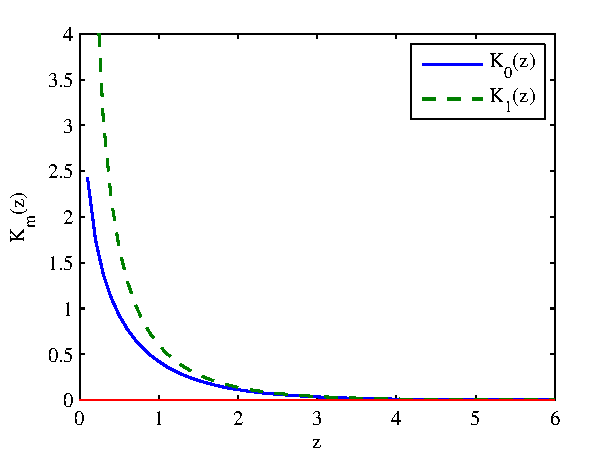
\includegraphics[width=\textwidth]{chp-2_bessel_k}
    (b) 子图b图题\\[0.3em]
    (b) Subfigure b
  \end{minipage}  \\
  \begin{minipage}[t]{0.5\textwidth}
    \centering
    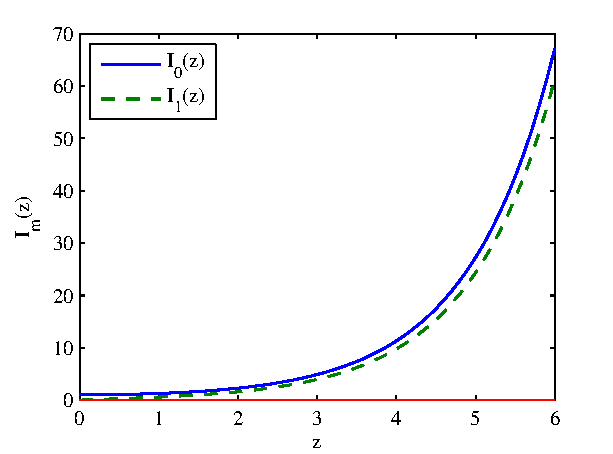
\includegraphics[width=\textwidth]{chp-2_bessel_i}
    (c) 子图c图题\\[0.3em]
    (c) Subfigure c
  \end{minipage}%
  \begin{minipage}[t]{0.5\textwidth}
    \centering
    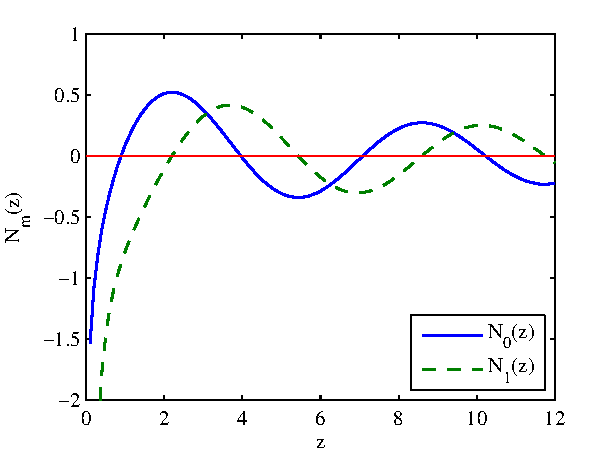
\includegraphics[width=\textwidth]{chp-2_bessel_n}
    (d) 子图d图题\\[0.3em]
    (d) Subfigure d
  \end{minipage}
  \FigureBiCaption{贝塞尔函数}{Bessel function} \label{fig-bessel-function}
\end{figure}

其它类似的多个图形并排或者堆叠均可以灵活的运用minipage照猫画虎获得。

\section{图题}\label{section2-4}
其实上边的例子中已经包含了图题的引用命令\verb|\FigureBiCaption|或命令\verb|\caption|两种方式,个人推荐使用第一种。
例如图 \ref{fig-bessel-function}中:
\begin{verbatim}
  \FigureBiCaption{贝塞尔函数}{Bessel function}\label{fig-bessel-function}
或
  \caption{贝塞尔函数\label{fig-bessel-function}}\vspace{0.3em}
  {Fig.  \ref{fig-bessel-function} Bessel function}
\end{verbatim}
为当前的图形添加中文图题“贝塞尔函数”,及英文图题“Bessel function”。同时添加标签“fig-bessel-function”。对图形的引用就是通过标签来实现的。

\section{图形的引用}\label{section2-5}
在已知图形的标签的基础之上,通过命令:
\begin{verbatim}
 \ref{label}
\end{verbatim}
来引用标签为“label”的图形。\LaTeX 会自动将其替换为图形的编号。例如:
\begin{verbatim}
贝塞尔函数的图形如图 \ref{fig-bessel-function}所示。
\end{verbatim}
的效果如下:\\
贝塞尔函数的图形如图 \ref{fig-bessel-function}所示。

\section{本章小结}\label{section2-6}
注意!从第二章开始应有``本章小结",主要总结本章所做的主要研究工作,研究成果等内容!!!

%

  % !Mode:: "TeX:UTF-8"
\chapter{表格}
\label{chap:table}

\section{普通三线表}\label{section3-1}
科技文献中常用的三线表:
\begin{table}[htbp!]
 \centering\small
  \TableBiCaption{燕山大学博士学位论文参考文献规则}{Reference rules of doctor degree theses of Yanshan university}\label{tab:ysubof}
 \begin{tabular}{llr}
 \toprule
    论文版本    & 参考文献标准    & 实施年份(年)  \\
 \midrule
    旧版        & BF7714-87       & 1987            \\
    新版        & GBT7714-2005    & 2005            \\
 \bottomrule
 \end{tabular}
\end{table}

实现代码如下:实现代码如下:实现代码如下:实现代码如下:实现代码如下:实现代码如下:实现代码如下:实现代码如下:实现代码如下:实现代码如下:实现代码如下:实现代码如下:
\begin{verbatim}
\begin{table}[htbp!]
\centering\small
\TableBiCaption{燕山大学博士学位论文参考文献规则}{Reference rules
of doctor degree theses of Yanshan university}\label{tab:ysubof}
\begin{tabular}{llr}
\toprule
论文版本    & 参考文献标准    & 实施年份(年)  \\
\midrule
旧版        & BF7714-87       & 1987            \\
新版        & GBT7714-2005    & 2005            \\
\bottomrule
\end{tabular}
\end{table}
\end{verbatim}

\section{有合并列的三线表}\label{section3-2}
合并列通常见于表格的第一行,在适当的位置使用\verb|\multicolumn| 命令即可。
\begin{table}[htbp!]
\centering\small
\TableBiCaption{带有合并列的三线表}{Three line table with a combined column}\label{tab:test}
\begin{tabular}{llr} \toprule
\multicolumn{2}{c}{Item} \\ \cmidrule(r){1-2}
Animal & Description & Price (\$)\\ \midrule
Gnat & per gram & 13.65 \\
& each & 0.01 \\
Gnu & stuffed & 92.50 \\
Emu & stuffed & 33.33 \\
Armadillo & frozen & 8.99 \\ \bottomrule
\end{tabular}
\end{table}


该表格是采用如下代码实现的:
\begin{verbatim}
\begin{table}[htbp!]
\centering\small
\TableBiCaption{带有合并列的三线表}{Three line table
with a combined column}\label{tab:test}
\begin{tabular}{llr} \toprule
\multicolumn{2}{c}{Item} \\ \cmidrule(r){1-2}
Animal & Description & Price (\$)\\ \midrule
Gnat & per gram & 13.65 \\
& each & 0.01 \\
Gnu & stuffed & 92.50 \\
Emu & stuffed & 33.33 \\
Armadillo & frozen & 8.99 \\ \bottomrule
\end{tabular}
\end{table}
\end{verbatim}

\section{表格的引用}\label{section3-3}
表格的引用同样是使用\verb|\ref{}| 命令实现的。例如“表\verb|\ref{tab:ysubof}|” 输出的结果为:表\ref{tab:ysubof}。

\section{特殊形式的表格}\label{section3-4}
\begin{verbatim}
\begin{table}[htbp!]
\centering\small
\TableBiCaption{中文}{English}\label{tab.2}
\begin{tabular*}{\columnwidth}{@{\extracolsep{\fill}}@{~~}cccccccc@{~~}}
\toprule
\multicolumn{7}{c}{ \hspace{2cm} The expected waiting queue length
$E({{L}_{q}})$}\\
\cline{2-8}
\raisebox{1ex}[0pt]{$\theta$}  &$p_2=0.1$     &$p_2=0.15$  &$p_2=0.2$
&$p_2=0.25$   &$p_2=0.3$  &$p_2=0.35$   &$p_2=0.4$\\
\midrule
0.3     &16.4830  &5.1232   &2.9232   &1.9704   &1.4339   &1.0886   &0.8479\\
0.5     &9.0488   &3.7848   &2.2906   &1.5839   &1.1723   &1.9035   &0.7146 \\
0.7     &7.4321   &3.3256   &2.0528   &1.4338   &1.0686   &0.8291   &0.6607 \\
\bottomrule
\end{tabular*}	
\end{table}
\end{verbatim}
生成
\begin{table}[htbp!]
	\centering\small
	\TableBiCaption{中文}{English}\label{tab.2}
	\begin{tabular*}{\columnwidth}{@{\extracolsep{\fill}}@{~~}cccccccc@{~~}}
		\toprule
		\multicolumn{7}{c}{ \hspace{2cm} The expected waiting queue length $E({{L}_{q}})$}\\
		\cline{2-8}
		\raisebox{1ex}[0pt]{$\theta$}  &$p_2=0.1$     &$p_2=0.15$  &$p_2=0.2$   &$p_2=0.25$   &$p_2=0.3$  &$p_2=0.35$   &$p_2=0.4$\\
		\midrule
		0.3     &16.4830  &5.1232   &2.9232   &1.9704   &1.4339   &1.0886   &0.8479\\
		0.5     &9.0488   &3.7848   &2.2906   &1.5839   &1.1723   &1.9035   &0.7146 \\
		0.7     &7.4321   &3.3256   &2.0528   &1.4338   &1.0686   &0.8291   &0.6607 \\
		\bottomrule
	\end{tabular*}	
\end{table}


\section{本章小结}\label{section3-5}
注意!从第二章开始应有``本章小结",主要总结本章所做的主要研究工作,研究成果等内容!!!


%

  % !Mode:: "TeX:UTF-8"
\chapter{公式}\label{chap:equ}

本章介绍基本公式的输入方法;矩阵和向量的输入;方程组的输入;多行公式的换行与对齐。
\LaTeX 中数学公式的输入依赖于数学环境。

在正文中用到的简短公式,可以直接使用两个美元符号“\$”括起来,如:
\begin{verbatim}
直角三角形三边长度满足关系式$a^2+b^2=c^2$。
\end{verbatim}
得到的结果是:\\
直角三角形三边长度满足关系式$a^2+b^2=c^2$。\\

而对于一些较为重要或者较复杂、需要编号的公式,则需要使用各种数学环境,例如使用equation环境:
\begin{verbatim}
\begin{equation}\label{chp-mode}
\mathbfit{E}=\mathrm{Re}(\mathbfit{E}(\mathbfit{r}))e^{j\omega t}.
\end{equation}
\end{verbatim}
得到的结果是:
\begin{equation}\label{chp-mode}
\mathbfit{E}=\mathrm{Re}(\mathbfit{E}(\mathbfit{r}))e^{j\omega t}.
\end{equation}
对它的引用方式为:\verb|公式 \eqref{chp-mode}|。\\
得到的结果为:公式 \eqref{chp-mode}。

如果不想对公式进行编号,则可以使用equation*环境:
\begin{verbatim}
\begin{equation*}\label{chp-m2}
\mathbfit{E}=\mathrm{Re}(\mathbfit{E}(\mathbfit{r}))e^{j\omega t}.
\end{equation*}
\end{verbatim}
得到的结果是:
\begin{equation*}\label{chp-m2}
\mathbfit{E}=\mathrm{Re}(\mathbfit{E}(\mathbfit{r}))e^{j\omega t}.
\end{equation*}

\section{上下标}\label{section4-1}
\verb|a_1+b^2\times c_1^2=0|输出结果为:$a_1+b^2\times c_1^2=0$。

\section{分式}\label{section4-2}
命令\verb|\frac, \dfrac\ tfrac|可以用来输出分式:
\begin{verbatim}
\begin{equation}\label{fr}
  \sin\dfrac{\cos\dfrac{a}{b}}{c}=
  \sin\frac{\cos\frac{a}{b}}{c}=
  \sin\tfrac{\cos\tfrac{a}{b}}{c}.
\end{equation}
\end{verbatim}
输出的结果是:
\begin{equation}\label{fr}
\sin\dfrac{\cos\dfrac{a}{b}}{c}=
\sin\frac{\cos\frac{a}{b}}{c}=
\sin\tfrac{\cos\tfrac{a}{b}}{c}.
\end{equation}

当使用括号来括起纵向尺寸较大的对象例如分式时,要使用\verb|\left| 和
\verb|\right| 命令使括号在纵向上伸长。例如:
\begin{verbatim}
\begin{equation}\label{frr}
  \left(\frac{a}{b}\right)=(\frac{a}{b}).
\end{equation}
\end{verbatim}
的输出结果是:
\begin{equation}\label{frr}
\left(\frac{a}{b}\right)=(\frac{a}{b}).
\end{equation}

\section{矢量点乘与叉乘}\label{section4-3}
矢量点乘:\verb|$\mathbfit{A}\cdot\mathbfit{B}$|输出:$\mathbfit{A}\cdot\mathbfit{B}$。

矢量叉乘:\verb|$\mathbfit{C}\times\mathbfit{D}$|输出:$\mathbfit{C}\times\mathbfit{D}$。

\section{求和与积分}\label{section4-4}
命令\verb|\sum|和命令\verb|\int|负责输出求和与积分号。例如:
\begin{verbatim}
\begin{equation}\label{equ-sum}
  \sum_{i=1}^n\sin\beta_i^2=0.
\end{equation}
\end{verbatim}
输出结果为:
\begin{equation}\label{equ-sum}
\sum_{i=1}^n\sin\beta_i^2=0.
\end{equation}
\begin{verbatim}
\begin{equation}\label{equ-int}
  \int_a^b\frac{c}{d}\,\mathrm{d}x=0.
\end{equation}
\end{verbatim}
输出结果为:
\begin{equation}\label{equ-int}
  \int_a^b\frac{c}{d}\,\mathrm{d}x=0.
\end{equation}


\section{矩阵与数组}\label{section4-5}
矩阵与数组使用array环境:
\begin{verbatim}
\begin{equation}\label{equ-array}
  \left(
    \begin{array}{c} a \\ c \end{array}
  \right)=
  \left(
    \begin{array}{cc} a & b \\ c & d \end{array}
  \right).
\end{equation}
\end{verbatim}
输出结果是:
\begin{equation}\label{equ-array}
  \left(
  \begin{array}{c} a \\ c \end{array}
  \right)=
  \left(
  \begin{array}{cc} a & b \\ c & d \end{array}
  \right).
\end{equation}
也可以使用matrix环境:
\begin{verbatim}
\begin{equation}\label{equ-matrix}
  \begin{matrix} 0 & 1 \\ 1 & 0\end{matrix}=
  \begin{pmatrix}0 &-i \\ i & 0\end{pmatrix}=
  \begin{bmatrix}1 & 0 \\ 0 &-1\end{bmatrix}=
  \begin{vmatrix}a & b \\ c & d\end{vmatrix}.
\end{equation}
\end{verbatim}
输出结果是:
\begin{equation}\label{equ-matrix}
  \begin{matrix} 0 & 1 \\ 1 & 0\end{matrix}=
  \begin{pmatrix}0 &-i \\ i & 0\end{pmatrix}=
  \begin{bmatrix}1 & 0 \\ 0 &-1\end{bmatrix}=
  \begin{vmatrix}a & b \\ c & d\end{vmatrix}.
\end{equation}

\section{多行公式与对齐方法}\label{section4-6}
多行公式排列,每个公式都有自己的编号通常使用align环境。例如:
\begin{verbatim}
\begin{align}
  a_1+a_2+a_3 &=0, \label{equ-s1}\\
  b_1+b_2+b_3+b_4 &=0, \label{equ-s2}\\
  c_1+c_2 &=0. \label{equ-v1}
\end{align}
\end{verbatim}
输出结果为:
\begin{align}
  a_1+a_2+a_3 &=0, \label{equ-s1}\\
  b_1+b_2+b_3+b_4 &=0, \label{equ-s2}\\
  c_1+c_2 &=0. \label{equ-v1}
\end{align}
其中符号“\&”为对齐符号。这里实现了等号对齐。

也可以使用eqnarray环境输入
\begin{verbatim}
\begin{eqnarray}
  a_1+a_2+a_3 &=&0, \label{equ-s1a}\\
  b_1+b_2+b_3+b_4 &=&0, \label{equ-s2a}\\
  c_1+c_2 &=&0. \label{equ-v1a}
\end{eqnarray}
\end{verbatim}
得到效果如下:
\begin{eqnarray}
  a_1+a_2+a_3 &=&0, \label{equ-s1a}\\
  b_1+b_2+b_3+b_4 &=&0, \label{equ-s2a}\\
  c_1+c_2 &=&0. \label{equ-v1a}
\end{eqnarray}

\section{带有大括号的方程组}\label{section4-7}
与多行公式不同,方程组左侧使用“\verb|\left{|”加了一个大括号,另外只有一个公式编号,因此采用equation和aligned结合的方式,例如:
\begin{verbatim}
\begin{equation}\label{equ-fml}
  \left\{
  \begin{aligned}
    x^2+y^2 &=0,\\
    x+y+z^2 &=0,\\
    x^2+y+z &=0.
  \end{aligned}
  \right.
\end{equation}
\end{verbatim}
输出结果为:
\begin{equation}\label{equ-fml}
  \left\{
  \begin{aligned}
    x^2+y^2 &=0,\\
    x+y+z^2 &=0,\\
    x^2+y+z &=0.
  \end{aligned}
  \right.
\end{equation}
也可以这样对齐,这样输入:
\begin{verbatim}
\begin{equation}\label{equ-fmla}
  \left\{
  \begin{array}{l}
    x^2+y^2 =0,\\
    x+y+z^2 =0,\\
    x^2+y+z =0.
  \end{array}
  \right.
\end{equation}
\end{verbatim}
得到的结果如下:
\begin{equation}\label{equ-fmla}
  \left\{
  \begin{array}{l}
    x^2+y^2 =0,\\
    x+y+z^2 =0,\\
    x^2+y+z =0.
  \end{array}
  \right.
\end{equation}

\section{特殊的公式}\label{section4-8}
\begin{verbatim}
$$
\bordermatrix{
& 0 & 1 & 2\cr
0 & A & B & C\cr
1 & d & e & f\cr
2 & 1 & 2 & 3},
$$
\begin{equation}
\bordermatrix{&a_1&a_2&...&a_n\cr
          b_1 & 1.2  & 3.3  & 5.1  & 2.8  \cr
          c_1 & 4.7  & 7.8  & 2.4  & 1.9  \cr
          ... & ...  & ...  & ...  & ...  \cr
          z_1 & 8.0  & 9.9  & 0.9  & 9.99  \cr}.
\end{equation}
\end{verbatim}
输出结果为:
$$
\bordermatrix{
& 0 & 1 & 2\cr
0 & A & B & C\cr
1 & d & e & f\cr
2 & 1 & 2 & 3},
$$
\begin{equation}
\bordermatrix{&a_1&a_2&...&a_n\cr
          b_1 & 1.2  & 3.3  & 5.1  & 2.8  \cr
          c_1 & 4.7  & 7.8  & 2.4  & 1.9  \cr
          ... & ...  & ...  & ...  & ...  \cr
          z_1 & 8.0  & 9.9  & 0.9  & 9.99  \cr}.
\end{equation}

\section{数学环境的使用}\label{section4-9}


一些常见的数学环境:
\begin{verbatim}
\theoremstyle{plain}
  \newtheorem{algo}{算法~}[chapter]
  \newtheorem{thm}{定理~}[chapter]
  \newtheorem{lem}[thm]{引理~}
  \newtheorem{prop}[thm]{命题~}
  \newtheorem{cor}[thm]{推论~}
\theoremstyle{definition}
  \newtheorem{defn}{定义~}[chapter]
  \newtheorem{conj}{猜想~}[chapter]
  \newtheorem{exmp}{例~}[chapter]
  \newtheorem{rem}{注~}
  \newtheorem{case}{情形~}
\theoremstyle{break}
  \newtheorem{bthm}[thm]{定理~}
  \newtheorem{blem}[thm]{引理~}
  \newtheorem{bprop}[thm]{命题~}
  \newtheorem{bcor}[thm]{推论~}
\renewcommand{\proofname}{\bf 证明}
\end{verbatim}

\subsection{定义}\label{defn}
\begin{verbatim}
\begin{defn}\label{defn4-1}
对于一些较为重要或者较复杂、需要编号的公式,则需要使用各种数学环境,例如使用equation环境:
得到的结果是:
\begin{equation}
\mathbfit{E}=\mathrm{Re}(\mathbfit{E}(\mathbfit{r}))e^{j\omega t}.
\end{equation}
  对它的引用方式为:\verb|公式 \eqref{chp-mode}|,
得到的结果为:公式 \eqref{chp-mode}。
\end{defn}
\end{verbatim}

\begin{defn}\label{defn4-1}
对于一些较为重要或者较复杂、需要编号的公式,则需要使用各种数学环境,例如使用equation环境:
得到的结果是:
\begin{equation}
\mathbfit{E}=\mathrm{Re}(\mathbfit{E}(\mathbfit{r}))e^{j\omega t}.
\end{equation}

对它的引用方式为:\verb|公式 \eqref{chp-mode}|,
得到的结果为:公式 \eqref{chp-mode}。
\end{defn}

\subsection{定理及证明}\label{thm}
\begin{verbatim}
\begin{thm}\label{theorem4-1}
对于一些较为重要或者较复杂、需要编号的公式,则需要使用各种数学环境,例如使用equation环境:得到的结果是:
\begin{equation}
\mathbfit{E}=\mathrm{Re}(\mathbfit{E}(\mathbfit{r}))e^{j\omega t}.
\end{equation}
  对它的引用方式为:\verb|公式 \eqref{chp-mode}|,
得到的结果为:公式 \eqref{chp-mode}。
\end{thm}
\begin{proof}
对于一些较为重要或者较复杂、需要编号的公式,则需要使用各种数学环境,例如使用equation环境。
\end{proof}
\end{verbatim}

\begin{thm}\label{theorem4-1}
对于一些较为重要或者较复杂、需要编号的公式,则需要使用各种数学环境,例如使用equation环境:得到的结果是:
\begin{equation}
\mathbfit{E}=\mathrm{Re}(\mathbfit{E}(\mathbfit{r}))e^{j\omega t}.
\end{equation}

对它的引用方式为:\verb|公式 \eqref{chp-mode}|,
得到的结果为:公式 \eqref{chp-mode}。
\end{thm}
\begin{proof}
对于一些较为重要或者较复杂、需要编号的公式,则需要使用各种数学环境,例如使用equation环境。
\end{proof}

\subsection{推论}\label{cor}
\begin{verbatim}
\begin{cor}\label{cor4-2}
推论推论推论推论推论推论推论:
对它的引用方式为:
得到的结果为:公式 \eqref{chp-mode}。
\end{cor}
\end{verbatim}

\begin{cor}\label{cor4-2}
推论推论推论推论推论推论推论:
对它的引用方式为:
得到的结果为:公式 \eqref{chp-mode}.
\end{cor}

\subsection{引理}\label{lem}
\begin{verbatim}
\begin{lem}\label{lemma4-2}
引理引理引理引理引理引理引理:对于一些较为重要或者较复杂、需要编号的公式,则需要使用各种数学环境,例如使用equation 环境:
\end{lem}
\end{verbatim}
\begin{lem}\label{lemma4-2}
引理引理引理引理引理引理引理:对于一些较为重要或者较复杂、需要编号的公式,则需要使用各种数学环境,例如使用equation 环境:
\end{lem}

\subsection{例子}\label{exmp}
\begin{verbatim}
\begin{exmp}\label{exmp4-2}
例例例例例例例例例例例例例例:
得到的结果是:
\begin{equation}
\mathbfit{E}=\mathrm{Re}(\mathbfit{E}(\mathbfit{r}))e^{j\omega t}.
\end{equation}
对它的引用方式为:\verb|公式 \eqref{chp-mode}|,
得到的结果为:公式 \eqref{chp-mode}。
\end{exmp}
\end{verbatim}
\begin{exmp}\label{exmp4-2}
例例例例例例例例例例例例例例:
得到的结果是:
\begin{equation}
\mathbfit{E}=\mathrm{Re}(\mathbfit{E}(\mathbfit{r}))e^{j\omega t}.
\end{equation}

对它的引用方式为:\verb|公式 \eqref{chp-mode}|,
得到的结果为:公式 \eqref{chp-mode}。
\end{exmp}

\section{本章小结}\label{section4-10}
注意!从第二章开始应有``本章小结",主要总结本章所做的主要研究工作,研究成果等内容!!!

%

  % !Mode:: "TeX:UTF-8"
\chapter{参考文献}
\label{chap:bib}

所有被引用的参考文献信息均存储在模板目录中的“bib”目录下,文件名为“tex.bib”。
由于使用了BibTeX,参考文献的格式是不需要手动调整。模板中的ysubst.bst 文件负责
文献格式输出。这里推荐您使用软件JabRef 来对文献进行管理。JabRef 支持中文,它可
以在这个网址下载到。\url{http://jabref.sourceforge.net/}

首先需要了解一个概念叫“BibTeX key”,也称作“BibTeX键”。它可以简单的理解为一篇
参考文献的“身份证号”。每一篇参考文献均有一个属于自己的不会重复的BibTeX key。
在引用文献的时候,需要使用引用命令\verb|\supercite{}|以上角标形式出现,使用引用命令\verb|\cite{}| 以正文形式出现。

\section{参考文献在正文和列表中格式要求}

\subsection{在正文中的要求}

在正文中,引用参考文献格式要求如下。

如果是单个作者的文献,应该写成:Kivshar\supercite {Kivshar2008}研究了...,得到了...结果。

如果是多个作者的文献,应该写成:Knight等\supercite{Knight1996}研究了...,得到了...结果。
姚建铨等\supercite{yaojianquan2009}研究了...,得到了...结果。只需要列出第一个作者加上``等''字即可。中英文的文献是一样的标准,都是加上`` 等''字。

文献的序号紧接着名字出现,而不是放到这句话的最后面,大家要统一一下。

\subsection{在列表中的要求}

参考文献的格式一定按照bib文件夹里的tex文件的格式书写,特别指出:

(1) 文献标识一定要加上,比如J、M、C、D等。

(2) 当三个以上作者是省略掉,只列出前三个,后边加上``等''、``et al''。

(3) 期刊的年、卷、期、页的格式:2018, 30(4): 15-30. 当缺少卷或期时,在参考文献tex.bib的文件里把相应的项不填就可以了。

上述指出的问题只要是严格按照模板格式去填写,就不会出现的。为了防止有上述不规范的情况出现,请打印装订之前务必检查是否有类似问题。


\section{单一参考文献}\label{section5-1}
例如这里我引用一篇文献:
\begin{verbatim}
Knight等\supercite{Knight1996}研究了...Russell是光子晶体光纤之父...。
\end{verbatim}
其中“Knight1996”是我要引用的文献的BibTeX 键。输出的结果为:

Knight等\supercite{Knight1996}研究了...Russell是光子晶体光纤之父...。

注意文献的编号是自动生成的,并且具有超链接功能。单击编号可以定位到文末的参考文献章节。

\section{多个连续参考文献}\label{section5-2}
 如果要一次引用多个文献,只要在引用命令中用英文逗号隔开各个BibTeX键即可,例如:
 \begin{verbatim}
我要引用2篇文献\supercite{Knight1996,Knight2000}。
\end{verbatim}
输出结果为:

我要引用2篇文献\supercite{Knight1996,Knight2000}。


如果是3 篇或者以上,加入更多BibTeX 键即可。例如:
 \begin{verbatim}
3篇文献\supercite{Knight1996,Knight2000,Knight2002}。
\end{verbatim}
输出结果为:

3篇文献\supercite{Knight1996,Knight2000,Knight2002}。

更多文献的例子:
 \begin{verbatim}
很多很多文献\supercite{Kivshar2008,John1987,Jing2010,Jeon2005,%
Jastrow2008,Jackson2008,Huttunen2005,Hou2008,Hilligsoe2004,%
Hassani2008,Han2002}。
\end{verbatim}

输出的结果为:很多很多文献\supercite{John1987,Jing2010,Jeon2005,%
Jastrow2008,Jackson2008,Huttunen2005,Hou2008,Hilligsoe2004,%
Hassani2008,Han2002}。



\section{多个不连续参考文献}\label{section5-3}
 \begin{verbatim}
四个不连续文献\supercite{Zhu2004,Zhu2001,Han2002,Knight1996}。
\end{verbatim}
四个不连续文献\supercite{Zhu2004,Zhu2001,Han2002,Knight1996}。

专利及学位论文格式如下:
\cite{jxz,Yu2004,Zhao2013}。

多个作者的中文文献显示如下\cite{yaojianquan2009},language=\{Chinese\}很重要,在bib文件中,中文文献要加上!会议论文的格式如下\cite{Li1998}。


\section{本章小结}\label{section5-4}
注意!从第二章开始应有``本章小结",主要总结本章所做的主要研究工作,研究成果等内容!!!

  % !Mode:: "TeX:UTF-8"
\chapter{数字物理量与单位}
\label{chap:unit}
模板加载了siunitx 宏包,可以实现长串数字位数的正确分割和各种物理量单位的自动格式化,避免
手工调用数学环境输入单位。尤其适用于理工科各种物理量的输入。该宏包的引入主要是为了解决论文
格式标准中的这个要求:
数字的书写不必每格一个数码,一般每两数码占一格,数字间分节不用分位号",",\emph{凡4位或4位以上的数都从个位起每3位数空\textbf{半个数码(1/4汉字)}。“\num{3 000000}”,不要写成}“3,000,000”,\emph{小数点后的数从小数点起向右按\textbf{每三位一组分节}。一个用阿拉伯数字书写的多位数不能从数字中间转行。}

\section{数字}\label{section7-1}
使用\verb|\num| 命令可以输入正确格式的长数字,包括科学计数法格式的数字。

\begin{table}[htbp]
\centering\zihao{5}
\TableBiCaption{siunitx 宏包与\LaTeX 数学环境输出效果对比}{Output effect comparison of siunitx macro package and \LaTeX\ mathematical environment}\label{tab.6a}
\begin{tabular}{ll|ll}
\toprule
siunitx 输出样式    & siunitx 输入方式          & \LaTeX 数学环境输出样式  & \LaTeX 数学环境输入方式     \\
\midrule
\num{123456789}     & \verb|\num{123456789}|    & 123456789             & \verb|123456789|         \\
\num{-1000000}      & \verb|\num{-1000000}|     & $-1000000$            & \verb|$-1000000$|        \\
\num{3.2e-8}        & \verb|\num{3.2e-8}|       & $3.2\times 10^{-8}$   & \verb|$3.2\times 10^{-8}$|\\
\num{1.2345678}     & \verb|\num{1.2345678}|    & 1.2345678             & \verb|1.2345678|          \\
\bottomrule
\end{tabular}
\end{table}


\section{单位}\label{section7-2}
单独输入单位时,可以采用\verb|\si|命令。

\begin{table}[htbp]
\centering\zihao{5}
\TableBiCaption{单位的不同输入方式}{Different input methods of units}\label{tab.6b}
\begin{tabular}{ll}
\toprule
输出样式  &输入方式     \\
\midrule
\si{kg.m/s^2}                           & \verb|\si{kg.m/s^2}|         \\
\si{g_{polymer}mol_{cat}.s^{-1}}       & \verb|\si{g_{polymer}mol_{cat}.s^{-1}}|\\
\si{\kilo\gram\metre\per\square\second} & \verb|\si{\kilo\gram\metre\per\square\second}|\\
\si{\gram\per\cubic\centi\metre}        &\verb|\si{\gram\per\cubic\centi\metre}|\\
\si{\square\volt\cubic\lumen\per\farad} &\verb|\si{\square\volt\cubic\lumen\per\farad}|\\
\si{\metre\squared\per\gray\cubic\lux}  &\verb|\si{\metre\squared\per\gray\cubic\lux}|\\
\si{\henry\second}                      &\verb|\si{\henry\second}|\\
\bottomrule
\end{tabular}
\end{table}

\section{同时输入数字与单位}\label{section7-3}

通常情况下,数字与单位是共同给出的,这时可以采用\verb|\SI| 命令。注意这里的 SI 是大写的。并且加入不同的可选项,最终的效果也不同。

\begin{table}[htbp]
\centering\zihao{5}
\TableBiCaption{同时输入数字与单位}{Numbers and units which are input at the same time}\label{tab.6c}
\begin{tabular}{ll}
\toprule
输出样式    & 输入方式  \\
\midrule
\SI[mode=text]{1.23}{J.mol^{-1}.K^{-1}}         & \verb|\SI[mode=text]{1.23}{J.mol^{-1}.K^{-1}}| \\
\SI{.23e7}{\candela}                            & \verb|\SI{.23e7}{\candela}|\\
\SI[per-mode=symbol]{1.99}[\$]{\per\kilogram}   & \verb|\SI[per-mode=symbol]{1.99}[\$]{\per\kilogram}|\\
\SI[per-mode=fraction]{1,345}{\coulomb\per\mole}& \verb|\SI[per-mode=fraction]{1,345}{\coulomb\per\mole}|\\
\bottomrule
\end{tabular}
\end{table}

\section{附1:国际标准单位与导出单位输入方式}\label{section7-4}

\begin{table}[htbp]
\centering\zihao{5}
\TableBiCaption{国际标准单位输入方式}{Unit input mode under International standard}\label{tab.6d}
\begin{tabular}{lllp{10pt}lll}
\toprule
单位    & 命令  & 符号  &   & 单位    & 命令  & 符号  \\
\midrule
安培    & \verb|\ampere|    & \si{\ampere}   && 坎德拉  & \verb|\candela|   & \si{\candela}  \\
开尔文  & \verb|\kelvin|    & \si{\kelvin}   && 千克    & \verb|\kilogram|  & \si{\kilogram}    \\
米      & \verb|\meter|     & \si{\meter}    && 摩尔    & \verb|\mole|      & \si{\mole}    \\
秒      & \verb|\second|    & \si{\second}   &&     &        &      \\
\bottomrule
\end{tabular}
\end{table}

\begin{table}[htbp]
\centering\zihao{5}
\TableBiCaption{国际标准导出单位输入方式}{Unit input mode which exported by International standard}\label{tab.6e}
\begin{tabular}{lllp{10pt}lll}
\toprule
单位    & 命令  & 符号  &   & 单位    & 命令  & 符号  \\
\midrule
becquerel       & \verb|\becquerel|     & \si{\becquerel}       & & newton      & \verb|\newton|    & \si{\newton} \\
degree Celsius  & \verb|\degreeCelsius| & \si{\degreeCelsius}   & & ohm         & \verb|\ohm|       & \si{\ohm}\\
coulomb         & \verb|\coulomb|       & \si{\coulomb}         & & pascal      & \verb|\pascal|    & \si{\pascal}\\
farad           & \verb|\farad|         & \si{\farad}           & & radian      & \verb|\radian|    & \si{\radian} \\
gray            & \verb|\gray|          & \si{\gray}            & & siemens     & \verb|\siemens|   & \si{\siemens}    \\
hertz           & \verb|\hertz|         & \si{\hertz}           & & sievert     & \verb|\sievert|   & \si{\sievert}\\
henry           & \verb|\henry|         & \si{\henry}           & & steradian   & \verb|\steradian| & \si{\steradian}\\
joule           & \verb|\joule|         & \si{\joule}           & & tesla       & \verb|\tesla|     & \si{\tesla}\\
katal           & \verb|\katal|         & \si{\katal}           & & volt        & \verb|\volt|      & \si{\volt}\\
lumen           & \verb|\lumen|         & \si{\lumen}           & & watt        & \verb|\watt|      & \si{\watt}\\
lux             & \verb|\lux|           & \si{\lux}             & & weber       & \verb|\weber|     & \si{\weber}\\
\bottomrule
\end{tabular}
\end{table}
%\section{附2:国际标准单位前缀}\label{section7-5}
%
%\begin{table}[htbp]
%\centering\zihao{5}
%\caption{国际标准单位前缀输入方式}
%\begin{tabular}{llllp{10pt}llll}
%\toprule
%名称    & 命令          & 符号          & 指数  &   & 名称      & 命令          & 符号      & 指数 \\
%\midrule
%yocto   & \verb|\yocto| & \si{\yocto}   & -24   &   & deca      &\verb|\deca|   &\si{\deca} & 1     \\
%zepto   & \verb|\zepto| & \si{\zepto}   & -21   &   & hecto     &\verb|\hecto|  &\si{\hecto}& 2\\
%atto    & \verb|\atto|  & \si{\atto}    & -18   &   & kilo      &\verb|\kilo|   &\si{\kilo} & 3\\
%femto   & \verb|\femto| & \si{\femto}   & -15   &   & mega      &\verb|\mega|   &\si{\mega} & 6\\
%pico    & \verb|\pico|  & \si{\pico}    & -12   &   & giga      &\verb|\giga|   &\si{\giga} & 9\\
%nano    & \verb|\nano|  & \si{\nano}    & -9    &   & tera      &\verb|\tera|   &\si{\tera} & 12\\
%micro   & \verb|\micro| & \si{\micro}   & -6    &   & peta      &\verb|\peta|   &\si{\peta} & 15\\
%milli   & \verb|\milli| & \si{\milli}   & -3    &   & exa       &\verb|\exa|    &\si{\exa}  & 18\\
%centi   & \verb|\centi| & \si{\centi}   & -2    &   & zetta     &\verb|\zetta|  &\si{\zetta}& 21\\
%deci    & \verb|\deci|  & \si{\deci}    & -1    &   & yotta     &\verb|\yotta|  &\si{\yotta}& 24\\
%\bottomrule
%\end{tabular}
%\end{table}


\section{本章小结}\label{section6-5}
注意!从第二章开始应有``本章小结",主要总结本章所做的主要研究工作,研究成果等内容!!!



%

  % !Mode:: "TeX:UTF-8"
%%%%%%% 以下内容不要修改!!! mzhy55
\makeatletter
\fancypagestyle{plain}{%
  \fancyhf{}%
  \renewcommand{\headrulewidth}{0pt}%
  \renewcommand{\footrulewidth}{0pt}%
%  \renewcommand{\headrule}{}
  \fancyhead[CE]{{\zihao{5} 燕山大学\CAST@value@degree 毕业设计(论文)}}
  \fancyhead[CO]{\zihao{5} 结\ \ 论}
  \fancyfoot[C]{{\zihao{-5} -~\thepage~-}}
  }
  \pagestyle{fancy}%%%%% 页眉 mzhy55
  \fancyhf{}
  \fancyhead[CE]{{\zihao{5} 燕山大学\CAST@value@degree 毕业设计(论文)}}
  \fancyhead[CO]{{\zihao{5} 结\ \ 论}}
  \fancyfoot[C]{{\zihao{-5} -~\thepage~-}}
\makeatother
%%%%%%% 以上内容不要修改!!! mzhy55

\begin{conclusion}
\label{chap:conclusion}

结论作为学位论文正文的组成部分,单独排写,不加章标题序号,不标注引用文献。结论内容一般在2000字以内。

结论应是作者在学位论文研究过程中所取得的创新性成果的概要总结,不能与摘要混为一谈。结论应包括论文的主要结果、创新点、展望三部分,在结论中应概括论文的核心观点,明确、客观地指出本研究内容的创新性成果(含新见解、新观点、方法创新、技术创新、理论创新),并指出今后进一步在本研究方向进行研究工作的展望与设想。对所取得的创新性成果应注意从定性和定量两方面给出科学、准确的评价,分(1)、(2)、(3)…条列出,宜用“提出了”、“建立了”等词叙述。此外,结论的撰写还应符合以下基本要求:

(1) 结论具有相对的独立性,不应是对论文中各章小结的简单重复。结论要与引言相呼应,以自身的条理性、明确性、客观性反映论文价值。对论文创新内容的概括,评价要适当。

(2) 结论措辞要准确、严谨,不能模棱两可,避免使用“大概”、“或许”、“可能是”等词语。结论中不应有解释性词语,而应直接给出结果。结论中一般不使用量的符号,而宜用量的名称。

(3) 结论应指出论文研究工作的局限性或遗留问题,如条件所限,或存在例外情况,或本论文尚难以解释或解决的问题。

(4) 常识性的结果或重复他人的结果不应作为结论。

\end{conclusion}


\renewcommand{\chaptermark}[1]{\markboth{附录~\thechapter~\hspace{0.5em}#1}{}} % 页眉上“附录”  mzhy55
  %% 附录
  \appendix
  %% !Mode:: "TeX:UTF-8"
\chapter{燕山大学研究生学位论文撰写规范}
\label{appendix}
% 重新定义 公式编号格式、图形、表格
\renewcommand\theequation{A-\arabic{equation}}
\renewcommand\thefigure{A-\arabic{figure}}
\renewcommand\thetable{A-\arabic{table}}


\begin{equation}\label{A1}
a=b^2+c_2.
\end{equation}

学位论文是研究生科学研究工作的全面总结,是表述其研究成果、代表其研究水平的重要学术文献资料,是申请和授予相应学位的基本依据。撰写学位论文是研究生培养的基本训练之一,必须按照规范认真执行。指导教师应加强指导,严格把关。
\begin{figure}[htbp]
\centering

\includegraphics[width=8cm]{ysulogo}
\caption{The Yanshan University LOGO}
\end{figure}\\
撰写的论文应符合国家及专业部门制定的有关标准,符合汉语语法规范。

硕士和博士学位论文除学术水平不同外,它们的撰写要求基本一致。

\begin{table}[htbp]
 \centering\zihao{5}
 \caption{燕山大学硕士学位论文参考文献规则}\label{tab:ysubof1}
 \begin{tabular}{llr}
 \toprule
    论文版本    & 参考文献标准    & 实施年份(年)  \\
 \midrule
    旧版        & BF7714-87       & 1987            \\
    新版        & GBT7714-2005    & 2005            \\
 \bottomrule
 \end{tabular}
\end{table}

\section{封面(封一、封皮)}\label{appendixA-1}

参见附录1学位论文封面示例。

封面格式参照附录1。各项名称的横向位置应居中安排,竖向间距按附录1安排。

开本尺寸,博士论文的为A4,装订切齐后为205×290mm;硕士论文的为B5,装订切齐后为178×250,单位为mm。

博士论文的书脊处应印:论文题目(小3号黑体,距上边线50mm)、姓名(距下边线30 mm)。

\section{封里(封二)}\label{appendixA-2}

博士、硕士学位论文的封里包括中文页及英文页。中、英文页的版式相同。对于博士、硕士等不同情况者的学位论文封里可参考附录2。

以研究生毕业同等学力申请学位者,需在封里的右上角加上如下字样:(同等学力人员)。

\section{摘要及关键词}\label{appendixA-3}

摘要是学位论文的必要附加部分,是以提供学位论文内容梗概为目的,不加评论和补充解释,简明、确切记述学位论文重要内容的完整短文。它反映了学位论文的精华。摘要应以浓缩的形式概括学位论文研究工作的目的、课题、基本观点、主要内容、研究方法及结论等。摘要应具有独立性和自明性,并拥有与学位论文同等量的主要信息,即不阅读学位论文全文就能获得必要的信息。

博士及硕士学位论文的摘要均要求用中、英两种文字给出,中文在前。

摘要的字数,以汉字计,硕士学位论文为500~650字;博士学位论文为900~1200字。摘要页不写论文题目。摘要中不宜使用公式、图表及参考文献序号。

摘要页的其它要求见附录3摘要及关键词示例。

关键词是为了适应计算机自动检索的需要,从论文中选取的能够反映文献特征内容的规范性词(称叙词或主题词)。应按GB3860-83《文献主题标引规则》的规定选取。对于那些反映新学科、新技术中的重要术语,也可作为关键词标出。关键词一般列5~10个,按词条外延层次从大到小排列。

\section{学位论文的组成部分和排列顺序}\label{appendixA-4}

学位论文一般由以下几个部分组成:封面、论文摘要、论文目录、正文、参考文献、
发表文章目录、致谢等。

\section{目录}\label{appendixA-5}

博士学位论文目录用中、英文给出,硕士学位论文目录只用中文给出。目录页的其它要求见附录4目录示例。

\section{正文}\label{appendixA-6}

\subsection{正文的内容}\label{appendixA-6-1}

正文由绪论、本论和结论三部分组成。

\subsubsection{绪论}\label{appendixA-6-1-1}

绪论是学位论文主体部分的开端,是全篇论文的引子。绪论主要回答``为什么研究(Why)"这个问题。它主要包括:

(1)研究的出发点与目的;

(2)研究的主要问题及范围,即研究主题简介;

(3)与学位论文有关的重要文献资料综述,相关领域前人及他人研究成果、水平和知识空白,存在的主要问题以及急待解决和完善的问题;

(4)理论分析依据,研究设想,研究方法和实验设计的概述;

(5)预期研究结果,科学意义和实用价值。

为了说明学位论文作者对研究方案的充分论证,反映作者在相关的学科领域中达到的学识水平以及具有开阔的科学视野,通常将文献综述作为绪论的重要内容。

综述用大量篇幅对本研究课题进行历史回顾,对前人和他人的研究工作及成果进行综合评述,然后引出自己的课题研究内容。综述相当于在学位论文研究领域内进行一次信息资料的专题研究报告。它反映了研究生阅读有关著作、学术期刊和文献资料的情况;也反应他所具备的基础和专业知识以及独立的自学能力。综述要求研究生对所阅读的文献资料进行消化、分析、判断和综合,决定取舍,确定自己所应开展科研工作的内容。只有在认真细致查阅参考文献的基础上,才能使自己的研究选题具有可靠的基础,尽量避免重复前人的研究工作,从而在前人的基础上解决前人没有解决或有待完善的工作。

撰写学位论文的绪论时,不要与摘要雷同,不要诠释基本理论,不要推导基本公式,不要介绍研究方法细节。写法应开门见山,言简意赅,措词精炼。

\subsubsection{本论}\label{appendixA-6-1-2}
本论是论文的主体部分,是作者研究成果的展示和表述。主要回答``怎么研究(how)"这个问题。它针对绪论部分提出的论点,全面透彻的进行分析论证,充分表达作者的见解。中心论点的论证可以从不同的角度展开,因此,可建立不同的分论点,共同围绕中心论点为其服务。

本论在安排层次上主要有三种方法:①递进式,即先提出一个论点,然后步步深入,层层展开,循序进行论述;②并列式,即把中心论点的几个从属论点并列起来,分别加以论述。③结合式,即把递进式和并列式结合在一起使用,这种方式多用于内容较多、篇幅较长的学位论文。层次可用小标题或序码表示。

本论的论证方法主要有:归纳分析法、演绎分析法、例证法、引证法、动因分析法、比较分析法、因素分析法、综合评析法等,可视情况灵活选用。

本论通常占学位论文的大部分篇幅。它的具体陈述方式往往不同学科有较大的差别,不能牵强地作出统一的规定。一般应在论文总体框架下按``概念的提出,理论的论证,方法的选择,试验的观察,数据的处理与分析,结果的检验"等,逐层分析,分章撰写。每一章的最后都要有``本章小结"。本章小结是用实践和数据给出的分析研究结果,最忌主观推测成分。
本
论要求思路清晰,合乎逻辑,用语简洁准确、明快流畅;内容务求客观、科学、完备,要尽量让事实和数据说话。凡是用简要的文字能够讲清楚的内容,应用文字陈述。用文字不容易说明白或说起来比较繁琐的,应用表或图来陈述。数据的引用要严谨确切,资料的引用要标明出处。

教科书式的撰写方法是撰写学位论文的第一大忌。对已有的知识避免重新描述和论证,尽量采用标注参考文献的方法;对用到的某些数学辅佐手段,应防止过分注意细节的数学推演,需要时可采用附录的形式收入学位论文供读者选阅。

\subsubsection{结论}\label{appendixA-6-1-3}
结论是指学位论文最终的总体结论。主要回答``研究出什么(what)"这个问题。它是在对本论分析、综合的基础上对全文的总结和升华,是对绪论和本论论点的呼应,是对全文的画龙点睛的收束,也是对本论中各章小结的再综合。可以作为结论的主要内容有:

(1)	本课题的理论、方法、设计计算和试验研究结果等的归纳和总结;

(2)	明确回答本研究课题所提出的问题和任务解决的程度和取得的进展;

(3)	明确指出本研究内容的创造性成果或创新点理论(含新观点、新思路、新见解)和方法;

(4)	对研究成果应用前景和社会、经济价值等加以预测和评价;

(5)	指出今后在本研究方向进一步开展研究工作的设想、展望和建议,仪器设备的改进,尚待解决的问题。

撰写结论时应注意的事项:

(1)	结论应该明确、精炼、完整、准确、措辞严密,不含糊其词;

(2)	结论要一分为二,要尊重前人的研究成果,实事求是的评价自己的成果,切勿言过其实,在无充分的把握时,应该留有余地。

(3)	结论应反映自己从事研究工作取得的成绩,属于前人或他人已有的正确结论,应不提或尽量少提。

结论应分条撰写,字数一般不多于2000字。


\subsection{正文的撰写要求}\label{appendixA-6-2}

\subsubsection{学位论文字数}\label{appendixA-6-2-1}
博士学位论文正文字数,理工科为8~12万字;管理及人文学科为10~14万字,其中绪论占一万字左右。

硕士学位论文正文字数,理工科为4~6万字,管理学科5~7万字(MBA3~4万字,案例分析论文不少于2万字),人文学科为3~5万字,外国语学科不少于2万外文词。其中绪论(人文学科为``导言",外国语学科为``引言Introduction")占3000~5000字。

\subsubsection{学位论文的版面要求}\label{appendixA-6-2-2}

(1) 页眉

页眉应居中置于页面上部。单数页眉的文字为``章及标题";双数页页眉的文字为``燕山大学硕士(博士)学位论文"。页眉的文字用5号宋体(文字上空一行书写)。页眉文字下面为两条横线(两条横线的长度与版芯尺寸相同,硕士论文线粗0. 5磅,博士论文线粗1.5磅)。

(2) 页码

摘要和目录的页码用罗马数字,正文的页码用阿拉伯数字,居中标于页面底部。正文部分的首页和翻开后的每一右页都应该是单数页码。研究生学位论文的原件要求用计算机排版、编辑与打印,余者可复印。

(3) 正文层次编排

建议采用表1所示格式,但若节下面无需列条者也可直接列款或项。

章标题用小2号黑体字,横向居中排放,竖向位置与目录页页题上、下留空相同,题序与题名间留一字空。

节标题用小3号黑体,条标题用4号黑体,款标题用小4号黑体,正文用小4号宋体字。

外国语学科论文应使用英文Times New Roman小4号体,不可使用花体字;书名、文献名等作品名称应使用斜体字,段落书写采用首行缩进格式。

各层次标题均不得置于页面的最后一行,即不允许``背题"。

博士学位论文开本为A4,页边距为设置:上下分别为3cm,左右分别为2.8cm;正文满页为30行,每行36个字,每页版面字数为1080,行间距为最小值22磅。硕士学位论文开本为B5,页边距为设置:上下分别为2.7cm和2.3cm,左右分别为2.2cm和2.2cm,正文满页为29行,每行32个字,每页版面字数为928,行间距为最小值20磅。

\subsubsection{引用文献}\label{appendixA-6-2-3}
正文中引用文献,应将所引用文献的编号(用阿拉伯数字的小4号字)括以方括号,置于所引内容最后一个字的右上角,如``二次铣削[1]"。当引用某文件的结论时,可将该文件编号用小4号字加方括号与正文排齐,如``由文献[8,10~14]可知"。

各级标题处均不得设置引用文献标示。

\subsubsection{名词术语}\label{appendixA-6-2-4}
科技名词术语及设备、元器件名称,应符合有关标准中的规定。标准中未予规定的术语、名词,应采用行业通用的。论文中自行采用的新名词(包括中、外文的)应加以注释。第一次出现的英文缩写应加括号标出全称。

\subsubsection{物理量的表示}\label{appendixA-6-2-5}
论文中表示物理量的名称和符号应执行GB3100~3102-86的规定(参见附录5)。物理量的符号都必须用斜体。

\subsubsection{计量单位}\label{appendixA-6-2-6}
物理量计量单位及符号应按国务院1984年发布的《中华人民共和国法定计量单位》及GB3100~3102《量和单位》系列国家标准(见附录5、6)执行,不得使用非法定计量单位及符号。

表达量时,在公式图表和文字叙述中,一律使用单位的国际符号。某些单位没有国际符号时,可用汉字与国际符号构成组合单位。如:m2/人,t/月。数值与单位符号间应留一个空格。
量符号必须采用斜体字母。矢量、张量符号一律用黑斜体。量符号下角标有斜体的,正体的和正体斜体混合的,要注意区分(见附录7)。

计量单位符号一律用正体。一般单位符号为小写体,只有来源于人名的单位,其符号的首字母大写。

词头是为了避免过大或过小的数值而加在SI单位之前构成十进倍数或分数单位的因数符号。

词头符号一律采用正体。表示因数符号大于106的词头符号为大写体,其余均为小写体。特别要注意区分Y(1024)和y(10-24)、Z(1021)和z(10-21)、P(1015)和p(10-12)、M(106)和m(10-3)。词头符号与单位符号之间不留空隙,也不加任何符号。

\subsubsection{数字}\label{appendixA-6-2-7}
按国家语言文字工作委员会等七单位1987年公布的《关于出版物上数字用法的执行规定》,除习惯用中文数字表示的以外,一般均采用阿拉伯数字(见附录8)。

\subsubsection{数理公式}\label{appendixA-6-2-8}
公式原则上应居中书写。比较简单的或叙述性的式子可以串文排。

公式序号按章编排,如第2章第1个公式为``(2-1)"。序号加圆括号,与公式同行排在右顶格处。

文中引用公式时,用``见式(1-1)或由公式(1-1)"。公式后若有说明文字,如``式中……",应另起一行,左起顶格排放。

为了节省版面,便于转行或减少排版难度,要对公式采用合理的表达形式,如 和 , 和 , 和 等,采用后者较方便。
公式转行容易出错。需要转行时,最好参阅一下数理公式的转行规则(见附录9)。

\subsubsection{插表}\label{appendixA-6-2-9}
学位论文中表格的运用是比较多的。表格能够增强表述内容的逻辑性和准确性,已成为现代科技文献中不可缺少的表述手段。使用合适的表格,将使论文的篇幅紧凑、论述清晰,给人以强烈的对比效果。
一个表格应尽量保持完整,没有特殊需要不要分割成两部分或更多部分。表格的位置安排,一般应随文列出,要紧接在第一次涉及它的文字段后面,应尽量与涉及文字在同一段落,或编排在同一页码上。但有时限于论文结构,或表格容量较大,也可以把表格放在涉及文字段落稍后的地方,这时仍然应该争取与涉及的文字段落放在同一章节和同一个视页中。必要时,表格也可分为两段或多段(这只能发生在转页时),转页分段后的每一续表的表头都应重新排字,重排表头的续表起始横线上方居中应注明``续表 "字样。

有些表宽大于版芯的表格,需要左转90o排,这时表头一律朝左(即单页上朝钉口,双页上朝切口),表底一律朝右。少数容量特别大的表格需要跨页排时,应尽量采用双页跨单页底骑缝表方式(避免单跨双的转面表),以使整个表格呈现在一个视野上。
表格不加左右边线,上、下边线为粗实线(1.5磅)。

表格均应有表题(由表序和表名组成)。表序编排规则与公式符号的一样。表序与表名之间空一格,表名中和表名后均不使用标点符号。表题置于表上,居中排放。表题要求用中、英两种文字,中文在上,中、英文表题以及表题与表格间距为最小值18磅。工程硕士学位论文不要求英文表题。
全表如用同一单位,应将单位符号移至表头右上角,加圆括号(见附录10中例2)。

表内数字空缺的格内加横线``-"(占两个数字宽度)。表内文字或数字上、下或左、右相同时,采用通栏处理方式(见附录10中例2),不允许使用``〃"、``同上"之类的写法。

表内文字说明,起行空一格,转行顶格,句末不加标点。表题用5号字,表内文字及表的说明文字均用小5号字,英文用正体,中文用宋体。

\subsubsection{插图}\label{appendixA-6-2-10}
学位论文中的插图与文字一样是用来表达作者意图的有效工具。插图可以形象、直观地表述科学思想和技术内容,被称为``形象语言",插图可以使某些内容的描述简洁、清晰,可省略大段文字,有利于紧缩篇幅。
插图重要特点是它的原始设计,应由论文作者自己来完成。设计插图时应注意图形的示意性;内容的写实性;取舍的灵活性和绘制的规范性。插图的线条粗细与插图的大小有关,插图大线条粗些,插图小线条细些,要保持整篇论文插图线条的统一。
论文中使用的机械工程图应符合GB4457~GB131-83《机械制图》标准规定;电气图应符合附录11所列有关标准的规定;流程图原则上应采用结构化程序并正确运用流程框图。对于无规定符号的图,应采用相应行业上的常用画法。
每个图均应有图题(由图号和图名组成)。图号编排同表序编排规定。图题置于图下,表题用中、英文两种文字居中排放。中文的在上。文字与图的竖向间距同插表。图名在图号之后空一字排放。引用图要在图题右上角加引用的文献号。图中若有分图时,分图图题也置于分图之下,分图号用(a)、(b)等表示。分图应尽量横向排列,分图较宽者,可纵向排列,分图较多者,也可横、纵向组合排列。图宽大于版芯的图,需要左转90o排,单数页图题在切口边,双数页图题在钉口边。
图题用5号字,图内文字用小5号字。中文为宋体,英文为正体。工程硕士学位论文不要求英文图题。

论文中引入插图之前,必须有该插图的提示语,如``见图1-1"等。若提示语后面的版页不够排放该图时,则可将图后部分文字提到图前排版,将该图移到次页最上端或次页首段末。


\subsubsection{照片图}\label{appendixA-6-2-11}
学位论文原件中照片图应采用原版照片(黑白、彩色均可)粘贴,不得用复印图。照片采用光面相纸不用布纹相纸。对金相显微组织照片必须注明放大倍数。

学位论文原件中的插图也不得用复印件。对于复杂的引用图,可采用数字化仪输入计算机打印出来的图。

\section{附录}\label{appendixA-7}

附录是学位论文的附件,不是必要组成部分。对需要收录于学位论文中且又不适
合置于正文的附加数据、资料、公式推导,程序等内容,可做为附录排在``结论"和``参考文献"之间,序号采用``附录1"、``附录2"等,采用小2号黑体字,左侧顶格开排,纵向位置同``目录"

\section{参考文献}\label{appendixA-8}

在学位论文中收录参考文献具有多方面的作用:1)对他人研究成果的尊重;2)
提供阅读学位论文的参考资料;3)表明学位论文中所引资料的可信度;4)便于他人参阅从事进一步研究。

(1)	准确恰当地引用和标注参考文献有助于提高学位论文的学术水平。
 撰写学位论文都必然涉及到对本领域前人或他人研究成果的比较、分析、综合
或者运用,以便用来支持和丰富自己的学位论文。准确恰当地引用和标注参考文献,有助于反映学位论文的学术背景、研究目的和研究深度;有助于反映学位论文作者的科学态度和科学依据;有助于说明研究方法或过程的合理性以及研究结果的可靠性;有助于明确本人研究与前人研究的关系,突出学位论文的创新或独到之处;有助于明晰学位论文和所引用文献的著作权关系,避免因为漏引、误引或标注不清所引起的抄袭或者剽窃之嫌。

(2)	准确恰当地引用和标注参考文献是科学研究工作者的职业道德。
 既是对前人或他人劳动成果的尊重,又是对提高学位论文的学术质量有水涨船
高之效。

(3)	准确恰当地引用和标注参考文献是对参考文献作者的尊重。
故意把他人作品中的成果(说法、公式、数据、结论等)当作自己的而不加以说
明,视为抄袭或剽窃行为。

(4)	准确恰当地引用和标注参考文献是培养研究生树立知识产权意识的一项技
术性很强的工作。

    参考文献书写格式应符合BF7714-87《文后参考文献著录规则》。常用参考文献编写项目和顺序规定如下:

          著作图书文献
  序号    作者.书名.版次.出版地:出版者,出版年:引用部分起止页
                                                         第一版应省略
          翻译图书文献
  序号    作者.书名.译者.版次.出版地:出版者,出版年:引用部分起止页
                                                         第一版应省略
          学术刊物文献
  序号    作者.文章名.学术刊物名,年,卷(期):引用部分起止页
          学术会议文献
  序号    作者.文章名.编者名.会议名称,会议地址,年份.出版地,出版者,出版年:引用         部分起止页
           学位论文类参考文献
  序号    研究生姓名.学位论文题目.[学校及学位论文级别].答辩年份:引用部分起止页(起止页码之间采用短横线``-"表示)

    学术会议若出版论文集者,可在会议名称后加上``论文集"字样。未出版论文集者省去``出版者"、``出版年"两项。会议地址与出版地相同者省略``出版地"。会议年份与出版年相同者省略``出版年"。
参考文献字号用5号宋体。参考文献书写格式见附录12参考文献示例。
博士学位论文的参考文献数一般应不少于100篇,其中外文文献一般不少于
总数的1/2;硕士学位论文的参考文献一般应不少于50篇,其中外文文献一般不少于20篇。参考文献中近五年的文献数一般应不少于总数的1/3,并应有近两年的参考文献。工程硕士学位论文的参考文献一般不应少于20篇。
人文学科的``参考文献部分"分为``注释"和``参考文献"两部分。其中"注释"采用脚注的形式。注释和参考文献总数要求在50篇以上,其中注释大于30篇,注释和参考文献中的外文文献不少于1/10。
外国语学科学位论文注释采用尾注的形式。

    产品说明书、各类标准、各种报纸上刊登的文章及未公开发表的研究报告(著名的内部报告如PB、AD报告及著名大公司的企业技术报告等除外)等通常不宜作为参考文献引用。
引用网上参考文献时,应注明该文献的准确网页地址,网上参考文献不包含在上述规定的文献数量之内。


\section{攻读学位期间承担的科研任务与主要成果}\label{appendixA-9}

该页页题为:攻读博(硕)士学位期间承担的科研任务与主要成果,其字体、字
号及横、纵向位置同参考文献页。该项的主要内容包括:

(1)	承担的研究课题;

(2)	科学研究成果(包括已发表的学术论文;研究报告;专著与教材;科研成果获奖项目等);

(3)	专利申报情况。

\section{致谢}\label{appendixA-10}

论文的最后一段写致谢,这是作者对论文的形成作过贡献的组织或个人予以感谢
的文字记载。致谢的对象主要有:

1.	对资助研究工作的基金会、合作单位、企业和个人表示谢意;

2.	对指导教师、答疑教师、实验教师以及协助完成研究工作的人员致谢;

3.	对论文撰写过程中提出建议和提供帮助的人员致谢;

4.	对学位论文引用过的资料、图表、文献、研究思想和设想的知识产权所有者表示感谢。

致谢不仅是一种礼貌,也是对他人劳动的尊重。致谢的内容要实在,语言要诚恳、恰当、简练;不应该借学位论文完成之机,对提供过与论文工作无关的其它帮助的人员致谢。

\section{索引}\label{appendixA-11}

为便于索引文中内容,可在论文``致谢"页后编排索引页(若无需要亦可不设索引页)。索引以论文中的专业词语为检索线索,指出其相关内容所在页码。索引设中、英两种文字页,中文页在前,中文页按名词汉语拼音第一个字母排序,英文按该词第一个英文字母排序。索引示例见附录13。

\section{作者简介}\label{appendixA-12}

所有学科的博(硕)士学位论文都要求附以``作者简介"页。左上角放置作者彩照(小2寸)。

作者简介包括的内容:姓名、性别、民族、籍贯。作者简历:大学毕业的时间、院校、专业、学位。主要工作单位及从事过的与本学位论文有关的工作。取得的科研成果:发表的学术论文、专著、教材。获奖情况及获国家专利情况等。

  % !Mode:: "TeX:UTF-8"
\makeatletter
\fancypagestyle{plain}{%
  \fancyhf{}%
  \renewcommand{\headrulewidth}{0pt}%
  \renewcommand{\footrulewidth}{0pt}%
%  \renewcommand{\headrule}{}
  \fancyhead[CE]{{\zihao{5} 燕山大学\CAST@value@degree 毕业设计(论文)}}
  \fancyhead[CO]{\zihao{5} \nouppercase \leftmark}
  \fancyfoot[C]{{\zihao{-5} -~\thepage~-}}
  }
  \pagestyle{fancy}%%%%% 页眉 mzhy55
  \fancyhf{}
  \fancyhead[CE]{{\zihao{5} 燕山大学\CAST@value@degree 毕业设计(论文)}}
  \fancyhead[CO]{{\zihao{5} \nouppercase \leftmark}}
  \fancyfoot[C]{{\zihao{-5} -~\thepage~-}}
\makeatother
%%%%%%% 以上内容不要修改!!! mzhy55

\chapter{程序代码的输入}
\label{appendixB}
% 重新定义 公式编号格式、图形、表格
\renewcommand\theequation{A-\arabic{equation}}
\renewcommand\thefigure{A-\arabic{figure}}
\renewcommand\thetable{A-\arabic{table}}

\begin{equation}\label{B1}
a=b^2+c_2.
\end{equation}

\section{插入程序代码}\label{appendixB-1}
\label{chap}

使用lisitings宏包可以在正文中插入程序的代码,插入的代码有自己的字体,可以实现行号、关键字高亮等功能。该环境的参数language决定了程序
的类型,例如\verb|language={[77]Fortran}|指定程序代码为FORTRAN语言;\verb|language={MATLAB}|指定程序代码为MATLAB的m语言。下边给出具体的例子。

\section{FORTRAN}\label{appendixB-2}

\begin{lstlisting}[language={[77]Fortran},
numbers=left,
numberstyle=\tiny,
basicstyle=\small\ttfamily,
stringstyle=\color{purple},
keywordstyle=\color{blue}\bfseries,
commentstyle=\color{brown},
frame=single]
C MATLAB gateway
      subroutine mexFunction(nlhs, plhs, nrhs, prhs)
C variables
      integer nlhs, nrhs
      integer plhs(*), prhs(*)
C input pointers
      pr_x=mxgetpr(prhs(1))
      pr_x1=mxgetpr(prhs(2))
C output pointers
      plhs(1)=mxCreateDoubleScalar(0)
      pr_y=mxGetPr(plhs(1))
C calculation
      call eim(%val(pr_x),%val(pr_x1),%val(pr_y))
      end subroutine mexFunction
\end{lstlisting}

\section{MATLAB}\label{appendixB-3}
\begin{verbatim}
\begin{lstlisting}[language={MATLAB},
numbers=left,
numberstyle=\tiny,
basicstyle=\small\ttfamily,
stringstyle=\color{purple},
keywordstyle=\color{blue}\bfseries,
commentstyle=\color{brown},
frame=single]
% bessel j

n=-0:0.1:12;
y=n*0;
b0n=besselj(0,n);
b1n=besselj(1,n);
plot(n,b0n,'-',n,b1n,'-',0:0.1:12,y)

ylabel('J_m(z)')
xlabel('z')
legend('J_0(z)','J_1(z)')
\end{lstlisting}
\end{verbatim}
输出的结果为:
\begin{lstlisting}[language={MATLAB},
numbers=left,
numberstyle=\tiny,
basicstyle=\small\ttfamily,
stringstyle=\color{purple},
keywordstyle=\color{blue}\bfseries,
commentstyle=\color{brown},
frame=single]
% bessel j

n=-0:0.1:12;
y=n*0;
b0n=besselj(0,n);
b1n=besselj(1,n);
plot(n,b0n,'-',n,b1n,'-',0:0.1:12,y)

ylabel('J_m(z)')
xlabel('z')
legend('J_0(z)','J_1(z)')
\end{lstlisting}

\section{C++}\label{appendixB-4}
\begin{verbatim}
\begin{lstlisting}[language={C++},
numbers=left,
numberstyle=\tiny,
basicstyle=\small\ttfamily,
stringstyle=\color{purple},
keywordstyle=\color{blue}\bfseries,
commentstyle=\color{brown},
frame=single]
# include{iostream.h}
void main()
int r;
double n;
{
cout<<"hello, LaTeX!"<<endl;
}
\end{lstlisting}
\end{verbatim}
输出的结果为:
\begin{lstlisting}[language={C++},
numbers=left,
numberstyle=\tiny,
basicstyle=\small\ttfamily,
stringstyle=\color{purple},
keywordstyle=\color{blue}\bfseries,
commentstyle=\color{brown},
frame=single]
# include{iostream.h}
void main()
int r;
double n;
{
cout<<"hello, LaTeX!"<<endl;
}
\end{lstlisting}



% 以下为附件部分
%----------------------------%
\backmatter
  \renewcommand{\chaptermark}[1]{\markboth{#1}{}} % 页眉上“参考文献、成果、致谢” mzhy55
%%%%%%% 以下内容不要修改!!! mzhy55
\makeatletter
\fancypagestyle{plain}{%
  \fancyhf{}%
  \renewcommand{\headrulewidth}{0pt}%
  \renewcommand{\footrulewidth}{0pt}%
%  \renewcommand{\headrule}{}
\fancyhead[CE]{{\zihao{5} 燕山大学\CAST@value@degree\CAST@label@thesis}}
\fancyhead[CO]{\zihao{5} 参考文献}
\fancyfoot[C]{{\zihao{-5} -~\thepage~-}}
}
\pagestyle{fancy}%%%%% 页眉 mzhy55
\fancyhf{}
\fancyhead[CE]{{\zihao{5} 燕山大学\CAST@value@degree\CAST@label@thesis}}
\fancyhead[CO]{{\zihao{5} 参考文献}}
\fancyfoot[C]{{\zihao{-5} -~\thepage~-}}
\makeatother
%%%%%%% 以上内容不要修改!!! mzhy55

  % 参考文献
  %|- 使用 BibTeX
    \bibliography{bib/参考文献}
    %\nocite{*}
  %|-不使用 BibTeX
    %
\begin{thebibliography}{10}

\bibitem{deng:01a}
{�˽���,~��ȽȽ,~�³���}.
\newblock {\em Computer Modern Typefaces}, volume~1 of {\em Computers and
Typesetting}.
\newblock ��ѧ������,~���:~7-03-009239-2/TP.1516, ����, 2001.

\bibitem{wang:00a}
����.
\newblock {\em Computer Modern Typefaces}, volume~2 of {\em Computers and
Typesetting}.
\newblock 2000.

\bibitem{zhang:03a}
���ֲ�.
\newblock {\em Computer Modern Typefaces}, volume~3 of {\em Computers and
Typesetting}.
\newblock 2003.

\bibitem{lshort-cn}
C\TeX{} ������.
\newblock {\em Computer Modern Typefaces}, volume~4 of {\em Computers and
Typesetting}.
\newblock 2003.

\bibitem{knuth86e}
Donald~E. Knuth.
\newblock {\em Computer Modern Typefaces}, volume~E of {\em Computers and
  Typesetting}.
\newblock Addison-Wesley, Reading, Massachusetts, 1986.

\bibitem{knuth86d}
Donald~E. Knuth.
\newblock {\em {METAFONT}: The Program}, volume~D of {\em Computers and
  Typesetting}.
\newblock Addison-Wesley, Reading, Massachusetts, 1986.

\bibitem{knuth86c}
Donald~E. Knuth.
\newblock {\em The {METAFONT}book}, volume~C of {\em Computers and
  Typesetting}.
\newblock Addison-Wesley, Reading, Massachusetts, 1986.

\bibitem{knuth86b}
Donald~E. Knuth.
\newblock {\em {TeX}: The Program}, volume~B of {\em Computers and
  Typesetting}.
\newblock Addison-Wesley, Reading, Massachusetts, 1986.

\bibitem{knuth86a}
Donald~E. Knuth.
\newblock {\em The {TeX}book}, volume~A of {\em Computers and Typesetting}.
\newblock Addison-Wesley, Reading, Massachusetts, 1986.

\bibitem{lamport85a}
Leslie Lamport.
\newblock {\em {LaTeX} --- A Document Preparation System: User's Guide and
  Reference Manual}.
\newblock Addison-Wesley, Reading, Massachusetts, 2nd edition, 1985.

\end{thebibliography}


  % 发表文章目录
  %% !Mode:: "TeX:UTF-8"
\makeatletter
\fancypagestyle{plain}{%
  \fancyhf{}%
  \renewcommand{\headrulewidth}{0pt}%
  \renewcommand{\footrulewidth}{0pt}%
%  \renewcommand{\headrule}{}
  \fancyhead[CE]{{\zihao{5} 燕山大学\CAST@value@degree 毕业设计(论文)}}
  \fancyhead[CO]{\zihao{5} 攻读硕士学位期间承担的科研任务与主要成果}
  \fancyfoot[C]{{\zihao{-5} -~\thepage~-}}
  }
  \pagestyle{fancy}%%%%% 页眉 mzhy55
  \fancyhf{}
  \fancyhead[CE]{{\zihao{5} 燕山大学\CAST@value@degree 毕业设计(论文)}}
  \fancyhead[CO]{{\zihao{5} 攻读硕士学位期间承担的科研任务与主要成果}}
  \fancyfoot[C]{{\zihao{-5} -~\thepage~-}}
\makeatother
%%%%%%% 以上内容不要修改!!! mzhy55

\begin{achievement}

%%%下列各项要按一、二、三、四...的顺序,没有的项要注释掉,后边的项序号相应调整!!!如果还有其它项可以类似的方式添加!!!   %%%mzhy55
%%%%%%%%%%%%%%%%%%%%%%%%%%%%%%%%%%%%%%%%%%%%\project
{\noindent\textbf{(一) 参与的科研项目}}    % 无科研项目时此项不必列出
\begin{enumerate}\setlength{\itemsep}{-0.4em}\zihao{5}%%%%%%%这一行的设定不要修改!!!
\renewcommand{\labelenumi}{[\theenumi]}
\item ×××, ×××. 人足机构学仿生与生物融合机构系统研究, 国家自然科学基金资助项目, 项目编号: 50675191.
\item ×××, ×××. 双重驱动少自由度并联机构型综合理论与应用, 河北省自然科学基金资助项目, 项目编号: E2009000388.
\item $\cdots$
\end{enumerate}


%%%%%%%%%%%%%%%%%%%%%%%%%%%%%%%%%%%%%%%%%%%%\publications
{\noindent\textbf{(二) 发表的学术论文}}    % 无学术论文时此项不必列出
\begin{enumerate}\setlength{\itemsep}{-0.4em}\zihao{5}%%%%%%%这一行的设定不要修改!!!
\renewcommand{\labelenumi}{[\theenumi]}
\item ×××, ×××, ×××. Optimization of Dispersion Properties of Photonic Crystal Fibers Using a Real-Coded Genetic Algorithm [J]. Chin. Phys. Lett., 2011, 28(6): 064215.
\item ×××, ×××. 并联2-RRR/UPRR踝关节康复机器人机构及其运动学 [J]. 机器人, 2010, 32(1): 6-12. (EI收录号: 20101212786168).
\item $\cdots$要与参考文献格式一致!!!
\end{enumerate}


%%%%%%%%%%%%%%%%%%%%%%%%%%%%%%%%%%%%%%%%%%%%%%%%%%%%%%%%%%%%%%%%%%%%%%%%%%%%%%%%%%%%%%
{\noindent\textbf{(三) 申请及已获得的专利}}    % 无专利时此项不必列出
\begin{enumerate}\setlength{\itemsep}{-0.4em}\zihao{5}%%%%%%%这一行的设定不要修改!!!
\renewcommand{\labelenumi}{[\theenumi]}
\item ×××, ×××. 具有远程运动中心的三自由度转动并联机构: 中国, 200910073844.8 [P]. 2011-01-05.
\item ×××, ×××. 五自由度双重驱动并联机构: 中国, 200910075071.7 [P]. 2011-01-05.
\end{enumerate}


%%%%%%%%%%%%%%%%%%%%%%%%%%%%%%%%%%%%%%%%%%%%%%%%%%%%%%%%%%%%%%%%%%%%%%%%%%%%%%%%%%%%%%
{\noindent\textbf{(四) 科研获奖}}    % 无奖励时此项不必列出
\begin{enumerate}\setlength{\itemsep}{-0.4em}\zihao{5}%%%%%%%这一行的设定不要修改!!!
\renewcommand{\labelenumi}{[\theenumi]}
\item ×××, ×××. 机器人机型综合及结构分析理论. XX省科学技术二等奖, 2009.
\end{enumerate}
\end{achievement}


  % 致谢
  %% !Mode:: "TeX:UTF-8"
\makeatletter
\fancypagestyle{plain}{%
  \fancyhf{}%
  \renewcommand{\headrulewidth}{0pt}%
  \renewcommand{\footrulewidth}{0pt}%
%  \renewcommand{\headrule}{}
  \fancyhead[CE]{{\zihao{5} 燕山大学\CAST@value@degree 毕业设计(论文)}}
  \fancyhead[CO]{\zihao{5} 致\ \ 谢}
  \fancyfoot[C]{{\zihao{-5} -~\thepage~-}}
  }
  \pagestyle{fancy}%%%%% 页眉 mzhy55
  \fancyhf{}
  \fancyhead[CE]{{\zihao{5} 燕山大学\CAST@value@degree 毕业设计(论文)}}
  \fancyhead[CO]{{\zihao{5} 致\ \ 谢}}
  \fancyfoot[C]{{\zihao{-5} -~\thepage~-}}
\makeatother
%%%%%%% 以上内容不要修改!!! mzhy55

\begin{thanks}
衷心感谢导师×××教授对本人的精心指导。他的言传身教将使我终生受益。

感谢×××教授,以及实验室全体老师和同窗们的热情帮助和支持!

本课题承蒙××××基金资助,特此致谢。

…

\end{thanks}


%  % 作者简介
%  % !Mode:: "TeX:UTF-8"
\begin{resume}
\vspace*{\baselineskip}
\noindent
\begin{minipage}[t]{4cm}
\vspace{-\baselineskip}

\includegraphics[width=3.3cm]{biophoto1}
\end{minipage}%
\hfill%
\begin{minipage}[t]{13cm}
\vspace{-\baselineskip}
%===============================
姓\qquad 名:×××

性\qquad 别:×

民\qquad 族:×族

出生年月:×××× 年× 月

籍\qquad 贯:××××
%===============================
\end{minipage}
\vspace*{\baselineskip}
%===============================

\textbf{学习经历}   % 自大学起

×××× 年× 月考入××大学××院××专业,×××× 年× 月本科毕业并获得××学士学位。

×××× 年× 月-- ×××× 年× 月,在燕山大学××学院××学科学习。

\textbf{获奖情况}   % 自大学起

×××× -- ×××× 年,燕山大学校级三好学生

×××× -- ×××× 年,燕山大学校级一等奖学金

×××× -- ×××× 年,燕山大学××学院三好学生

×××× -- ×××× 年,燕山大学××学院优秀团干部

(不含科研学术获奖)。

\textbf{工作经历}   % 没有可不写(将本行删除即可)

\end{resume}



\end{document}
%%===========================%
%% 全文结束
